\documentclass{book}
\usepackage[a4paper,top=2.5cm,bottom=2.5cm,left=2.5cm,right=2.5cm]{geometry}
\usepackage{makeidx}
\usepackage{natbib}
\usepackage{graphicx}
\usepackage{multicol}
\usepackage{float}
\usepackage{listings}
\usepackage{color}
\usepackage{ifthen}
\usepackage[table]{xcolor}
\usepackage{textcomp}
\usepackage{alltt}
\usepackage{ifpdf}
\ifpdf
\usepackage[pdftex,
            pagebackref=true,
            colorlinks=true,
            linkcolor=blue,
            unicode
           ]{hyperref}
\else
\usepackage[ps2pdf,
            pagebackref=true,
            colorlinks=true,
            linkcolor=blue,
            unicode
           ]{hyperref}
\usepackage{pspicture}
\fi
\usepackage[utf8]{inputenc}
\usepackage{mathptmx}
\usepackage[scaled=.90]{helvet}
\usepackage{courier}
\usepackage{sectsty}
\usepackage{amssymb}
\usepackage[titles]{tocloft}
\usepackage{doxygen}
\lstset{language=C++,inputencoding=utf8,basicstyle=\footnotesize,breaklines=true,breakatwhitespace=true,tabsize=4,numbers=left }
\makeindex
\setcounter{tocdepth}{3}
\renewcommand{\footrulewidth}{0.4pt}
\renewcommand{\familydefault}{\sfdefault}
\hfuzz=15pt
\setlength{\emergencystretch}{15pt}
\hbadness=750
\tolerance=750
\begin{document}
\hypersetup{pageanchor=false,citecolor=blue}
\begin{titlepage}
\vspace*{7cm}
\begin{center}
{\Large My Project }\\
\vspace*{1cm}
{\large Generated by Doxygen 1.8.2}\\
\vspace*{0.5cm}
{\small Fri Sep 21 2012 17:25:04}\\
\end{center}
\end{titlepage}
\clearemptydoublepage
\pagenumbering{roman}
\tableofcontents
\clearemptydoublepage
\pagenumbering{arabic}
\hypersetup{pageanchor=true,citecolor=blue}
\chapter{Namespace Index}
\section{Namespace List}
Here is a list of all documented namespaces with brief descriptions\-:\begin{DoxyCompactList}
\item\contentsline{section}{\hyperlink{namespace_krs}{Krs} }{\pageref{namespace_krs}}{}
\item\contentsline{section}{\hyperlink{namespace_krs_1_1_base}{Krs.\-Base} }{\pageref{namespace_krs_1_1_base}}{}
\item\contentsline{section}{\hyperlink{namespace_krs_1_1_base_1_1_logs}{Krs.\-Base.\-Logs} }{\pageref{namespace_krs_1_1_base_1_1_logs}}{}
\end{DoxyCompactList}

\chapter{Hierarchical Index}
\section{Class Hierarchy}
This inheritance list is sorted roughly, but not completely, alphabetically\-:\begin{DoxyCompactList}
\item Ado\-Net\-Appender\begin{DoxyCompactList}
\item \contentsline{section}{Krs.\-Base.\-Logs.\-Data\-Base\-Appender}{\pageref{class_krs_1_1_base_1_1_logs_1_1_data_base_appender}}{}
\end{DoxyCompactList}
\item \contentsline{section}{Krs.\-Base.\-Logs.\-Logger}{\pageref{class_krs_1_1_base_1_1_logs_1_1_logger}}{}
\item \contentsline{section}{Krs.\-Base.\-Logs.\-Log\-Message\-Helper}{\pageref{class_krs_1_1_base_1_1_logs_1_1_log_message_helper}}{}
\item \contentsline{section}{Krs.\-Base.\-Logs.\-Log\-Message\-Info}{\pageref{class_krs_1_1_base_1_1_logs_1_1_log_message_info}}{}
\item Pattern\-Layout\begin{DoxyCompactList}
\item \contentsline{section}{Krs.\-Base.\-Logs.\-Krs\-Layout}{\pageref{class_krs_1_1_base_1_1_logs_1_1_krs_layout}}{}
\end{DoxyCompactList}
\item Pattern\-Layout\-Converter\begin{DoxyCompactList}
\item \contentsline{section}{Krs.\-Base.\-Logs.\-Krs\-Message\-Pattern\-Converter}{\pageref{class_krs_1_1_base_1_1_logs_1_1_krs_message_pattern_converter}}{}
\end{DoxyCompactList}
\item \contentsline{section}{Krs.\-Base.\-Logs.\-Run\-Time\-Loger}{\pageref{class_krs_1_1_base_1_1_logs_1_1_run_time_loger}}{}
\end{DoxyCompactList}

\chapter{Class Index}
\section{Class List}
Here are the classes, structs, unions and interfaces with brief descriptions\-:\begin{DoxyCompactList}
\item\contentsline{section}{\hyperlink{class_krs_1_1_base_1_1_logs_1_1_data_base_appender}{Krs.\-Base.\-Logs.\-Data\-Base\-Appender} }{\pageref{class_krs_1_1_base_1_1_logs_1_1_data_base_appender}}{}
\item\contentsline{section}{\hyperlink{class_krs_1_1_base_1_1_logs_1_1_krs_layout}{Krs.\-Base.\-Logs.\-Krs\-Layout} \\*自定义布局,对自定义日志信息支持 }{\pageref{class_krs_1_1_base_1_1_logs_1_1_krs_layout}}{}
\item\contentsline{section}{\hyperlink{class_krs_1_1_base_1_1_logs_1_1_krs_message_pattern_converter}{Krs.\-Base.\-Logs.\-Krs\-Message\-Pattern\-Converter} \\*模式转换 }{\pageref{class_krs_1_1_base_1_1_logs_1_1_krs_message_pattern_converter}}{}
\item\contentsline{section}{\hyperlink{class_krs_1_1_base_1_1_logs_1_1_logger}{Krs.\-Base.\-Logs.\-Logger} }{\pageref{class_krs_1_1_base_1_1_logs_1_1_logger}}{}
\item\contentsline{section}{\hyperlink{class_krs_1_1_base_1_1_logs_1_1_log_message_helper}{Krs.\-Base.\-Logs.\-Log\-Message\-Helper} }{\pageref{class_krs_1_1_base_1_1_logs_1_1_log_message_helper}}{}
\item\contentsline{section}{\hyperlink{class_krs_1_1_base_1_1_logs_1_1_log_message_info}{Krs.\-Base.\-Logs.\-Log\-Message\-Info} \\*日志信息(\-Web) }{\pageref{class_krs_1_1_base_1_1_logs_1_1_log_message_info}}{}
\item\contentsline{section}{\hyperlink{class_krs_1_1_base_1_1_logs_1_1_run_time_loger}{Krs.\-Base.\-Logs.\-Run\-Time\-Loger} \\*计算执行时间差 }{\pageref{class_krs_1_1_base_1_1_logs_1_1_run_time_loger}}{}
\end{DoxyCompactList}

\chapter{Namespace Documentation}
\hypertarget{namespace_krs}{\section{Package Krs}
\label{namespace_krs}\index{Krs@{Krs}}
}
\subsection*{Namespaces}
\begin{DoxyCompactItemize}
\item 
package \hyperlink{namespace_krs_1_1_base}{Base}
\end{DoxyCompactItemize}

\hypertarget{namespace_krs_1_1_base}{\section{Package Krs.\-Base}
\label{namespace_krs_1_1_base}\index{Krs.\-Base@{Krs.\-Base}}
}
\subsection*{Namespaces}
\begin{DoxyCompactItemize}
\item 
package \hyperlink{namespace_krs_1_1_base_1_1_logs}{Logs}
\end{DoxyCompactItemize}

\hypertarget{namespace_krs_1_1_base_1_1_logs}{\section{Package Krs.\-Base.\-Logs}
\label{namespace_krs_1_1_base_1_1_logs}\index{Krs.\-Base.\-Logs@{Krs.\-Base.\-Logs}}
}
\subsection*{Classes}
\begin{DoxyCompactItemize}
\item 
class \hyperlink{class_krs_1_1_base_1_1_logs_1_1_data_base_appender}{Data\-Base\-Appender}
\item 
class \hyperlink{class_krs_1_1_base_1_1_logs_1_1_krs_layout}{Krs\-Layout}
\begin{DoxyCompactList}\small\item\em 自定义布局,对自定义日志信息支持 \end{DoxyCompactList}\item 
class \hyperlink{class_krs_1_1_base_1_1_logs_1_1_krs_message_pattern_converter}{Krs\-Message\-Pattern\-Converter}
\begin{DoxyCompactList}\small\item\em 模式转换 \end{DoxyCompactList}\item 
class \hyperlink{class_krs_1_1_base_1_1_logs_1_1_logger}{Logger}
\item 
class \hyperlink{class_krs_1_1_base_1_1_logs_1_1_log_message_helper}{Log\-Message\-Helper}
\item 
class \hyperlink{class_krs_1_1_base_1_1_logs_1_1_log_message_info}{Log\-Message\-Info}
\begin{DoxyCompactList}\small\item\em 日志信息(\-Web) \end{DoxyCompactList}\item 
class \hyperlink{class_krs_1_1_base_1_1_logs_1_1_run_time_loger}{Run\-Time\-Loger}
\begin{DoxyCompactList}\small\item\em 计算执行时间差 \end{DoxyCompactList}\end{DoxyCompactItemize}
\subsection*{Enumerations}
\begin{DoxyCompactItemize}
\item 
enum \hyperlink{namespace_krs_1_1_base_1_1_logs_aa1f948e33e410052b2716d8b68ec6583}{Log\-Level} \{ \hyperlink{namespace_krs_1_1_base_1_1_logs_aa1f948e33e410052b2716d8b68ec6583}{D\-E\-B\-U\-G} = 0, 
\hyperlink{namespace_krs_1_1_base_1_1_logs_aa1f948e33e410052b2716d8b68ec6583}{I\-N\-F\-O} = 1, 
\hyperlink{namespace_krs_1_1_base_1_1_logs_aa1f948e33e410052b2716d8b68ec6583}{E\-R\-R\-O\-R} = 3
 \}
\end{DoxyCompactItemize}


\subsection{Enumeration Type Documentation}
\hypertarget{namespace_krs_1_1_base_1_1_logs_aa1f948e33e410052b2716d8b68ec6583}{\index{Krs\-::\-Base\-::\-Logs@{Krs\-::\-Base\-::\-Logs}!Log\-Level@{Log\-Level}}
\index{Log\-Level@{Log\-Level}!Krs::Base::Logs@{Krs\-::\-Base\-::\-Logs}}
\subsubsection[{Log\-Level}]{\setlength{\rightskip}{0pt plus 5cm}enum {\bf Krs.\-Base.\-Logs.\-Log\-Level}}}\label{namespace_krs_1_1_base_1_1_logs_aa1f948e33e410052b2716d8b68ec6583}
\begin{Desc}
\item[Enumerator\-: ]\par
\begin{description}
\index{D\-E\-B\-U\-G@{D\-E\-B\-U\-G}!Krs\-::\-Base\-::\-Logs@{Krs\-::\-Base\-::\-Logs}}\index{Krs\-::\-Base\-::\-Logs@{Krs\-::\-Base\-::\-Logs}!D\-E\-B\-U\-G@{D\-E\-B\-U\-G}}\item[{\em 
\hypertarget{namespace_krs_1_1_base_1_1_logs_aa1f948e33e410052b2716d8b68ec6583}{D\-E\-B\-U\-G}\label{namespace_krs_1_1_base_1_1_logs_aa1f948e33e410052b2716d8b68ec6583}
}]调试日志 \index{I\-N\-F\-O@{I\-N\-F\-O}!Krs\-::\-Base\-::\-Logs@{Krs\-::\-Base\-::\-Logs}}\index{Krs\-::\-Base\-::\-Logs@{Krs\-::\-Base\-::\-Logs}!I\-N\-F\-O@{I\-N\-F\-O}}\item[{\em 
\hypertarget{namespace_krs_1_1_base_1_1_logs_aa1f948e33e410052b2716d8b68ec6583}{I\-N\-F\-O}\label{namespace_krs_1_1_base_1_1_logs_aa1f948e33e410052b2716d8b68ec6583}
}]信息日志 \index{E\-R\-R\-O\-R@{E\-R\-R\-O\-R}!Krs\-::\-Base\-::\-Logs@{Krs\-::\-Base\-::\-Logs}}\index{Krs\-::\-Base\-::\-Logs@{Krs\-::\-Base\-::\-Logs}!E\-R\-R\-O\-R@{E\-R\-R\-O\-R}}\item[{\em 
\hypertarget{namespace_krs_1_1_base_1_1_logs_aa1f948e33e410052b2716d8b68ec6583}{E\-R\-R\-O\-R}\label{namespace_krs_1_1_base_1_1_logs_aa1f948e33e410052b2716d8b68ec6583}
}]错误日志 \end{description}
\end{Desc}


\chapter{Class Documentation}
\hypertarget{class_krs_1_1_base_1_1_logs_1_1_data_base_appender}{\section{Krs.\-Base.\-Logs.\-Data\-Base\-Appender Class Reference}
\label{class_krs_1_1_base_1_1_logs_1_1_data_base_appender}\index{Krs.\-Base.\-Logs.\-Data\-Base\-Appender@{Krs.\-Base.\-Logs.\-Data\-Base\-Appender}}
}
Inheritance diagram for Krs.\-Base.\-Logs.\-Data\-Base\-Appender\-:\begin{figure}[H]
\begin{center}
\leavevmode
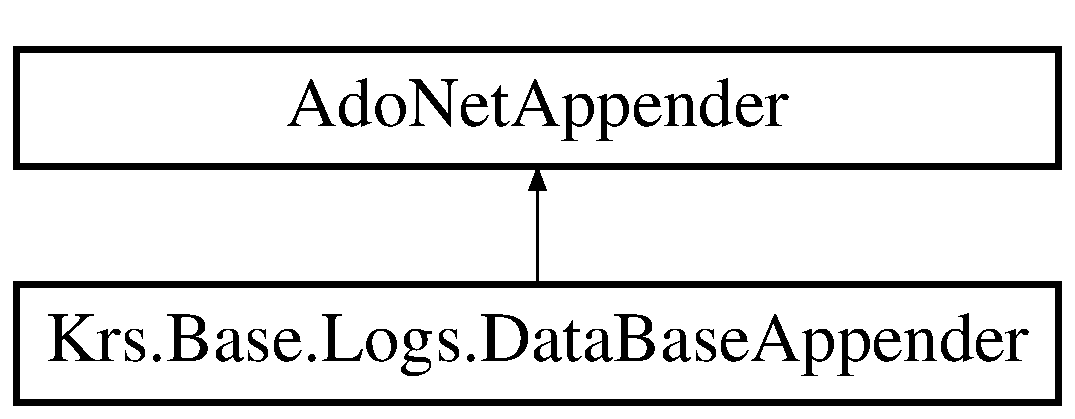
\includegraphics[height=2.000000cm]{class_krs_1_1_base_1_1_logs_1_1_data_base_appender}
\end{center}
\end{figure}
\subsection*{Public Member Functions}
\begin{DoxyCompactItemize}
\item 
\hypertarget{class_krs_1_1_base_1_1_logs_1_1_data_base_appender_acd39c06d7e9dbe893ab004baf1bf8acc}{override void {\bfseries Activate\-Options} ()}\label{class_krs_1_1_base_1_1_logs_1_1_data_base_appender_acd39c06d7e9dbe893ab004baf1bf8acc}

\item 
\hypertarget{class_krs_1_1_base_1_1_logs_1_1_data_base_appender_ac4491249a692ec3ec51637d717d2008f}{void {\bfseries Add\-Parameter} (Ado\-Net\-Appender\-Parameter parameter)}\label{class_krs_1_1_base_1_1_logs_1_1_data_base_appender_ac4491249a692ec3ec51637d717d2008f}

\end{DoxyCompactItemize}
\subsection*{Protected Member Functions}
\begin{DoxyCompactItemize}
\item 
\hypertarget{class_krs_1_1_base_1_1_logs_1_1_data_base_appender_aa7c0080eb6c1c473462082fc4062e1e8}{virtual string {\bfseries Get\-Log\-Statement} (Logging\-Event log\-Event)}\label{class_krs_1_1_base_1_1_logs_1_1_data_base_appender_aa7c0080eb6c1c473462082fc4062e1e8}

\item 
\hypertarget{class_krs_1_1_base_1_1_logs_1_1_data_base_appender_a2bfb14c67b2ab14a6e72caf33cd833e3}{override void {\bfseries On\-Close} ()}\label{class_krs_1_1_base_1_1_logs_1_1_data_base_appender_a2bfb14c67b2ab14a6e72caf33cd833e3}

\item 
\hypertarget{class_krs_1_1_base_1_1_logs_1_1_data_base_appender_ab4ddfb9e6d595f60b726110881c16b74}{virtual Type {\bfseries Resolve\-Connection\-Type} ()}\label{class_krs_1_1_base_1_1_logs_1_1_data_base_appender_ab4ddfb9e6d595f60b726110881c16b74}

\item 
\hypertarget{class_krs_1_1_base_1_1_logs_1_1_data_base_appender_a95ad583f03420bdd13cc7c8506332131}{override void {\bfseries Send\-Buffer} (Logging\-Event\mbox{[}$\,$\mbox{]} events)}\label{class_krs_1_1_base_1_1_logs_1_1_data_base_appender_a95ad583f03420bdd13cc7c8506332131}

\item 
\hypertarget{class_krs_1_1_base_1_1_logs_1_1_data_base_appender_ab50562553b5d20e455a9f4d7c9440180}{virtual void {\bfseries Send\-Buffer} (I\-Db\-Transaction db\-Tran, Logging\-Event\mbox{[}$\,$\mbox{]} events)}\label{class_krs_1_1_base_1_1_logs_1_1_data_base_appender_ab50562553b5d20e455a9f4d7c9440180}

\end{DoxyCompactItemize}
\subsection*{Properties}
\begin{DoxyCompactItemize}
\item 
\hypertarget{class_krs_1_1_base_1_1_logs_1_1_data_base_appender_a62c3718c52362c35b2784fa975dec81f}{string {\bfseries Command\-Text}\hspace{0.3cm}{\ttfamily  \mbox{[}get, set\mbox{]}}}\label{class_krs_1_1_base_1_1_logs_1_1_data_base_appender_a62c3718c52362c35b2784fa975dec81f}

\item 
\hypertarget{class_krs_1_1_base_1_1_logs_1_1_data_base_appender_af5e1b2e952b0414c278382e76b406b61}{Command\-Type {\bfseries Command\-Type}\hspace{0.3cm}{\ttfamily  \mbox{[}get, set\mbox{]}}}\label{class_krs_1_1_base_1_1_logs_1_1_data_base_appender_af5e1b2e952b0414c278382e76b406b61}

\item 
\hypertarget{class_krs_1_1_base_1_1_logs_1_1_data_base_appender_a4e9495c4b8ef7c885cf23055cc17f68b}{I\-Db\-Connection {\bfseries Connection}\hspace{0.3cm}{\ttfamily  \mbox{[}get, set\mbox{]}}}\label{class_krs_1_1_base_1_1_logs_1_1_data_base_appender_a4e9495c4b8ef7c885cf23055cc17f68b}

\item 
\hypertarget{class_krs_1_1_base_1_1_logs_1_1_data_base_appender_a0e8ba35df0ebbc35c343efc4a7138721}{string {\bfseries Connection\-String}\hspace{0.3cm}{\ttfamily  \mbox{[}get, set\mbox{]}}}\label{class_krs_1_1_base_1_1_logs_1_1_data_base_appender_a0e8ba35df0ebbc35c343efc4a7138721}

\item 
\hypertarget{class_krs_1_1_base_1_1_logs_1_1_data_base_appender_a35fa2e5fa410b16d554daca12c2858a4}{string {\bfseries Connection\-Type}\hspace{0.3cm}{\ttfamily  \mbox{[}get, set\mbox{]}}}\label{class_krs_1_1_base_1_1_logs_1_1_data_base_appender_a35fa2e5fa410b16d554daca12c2858a4}

\item 
\hypertarget{class_krs_1_1_base_1_1_logs_1_1_data_base_appender_aa1003c46f94e56fd273aea122a793fb7}{bool {\bfseries Reconnect\-On\-Error}\hspace{0.3cm}{\ttfamily  \mbox{[}get, set\mbox{]}}}\label{class_krs_1_1_base_1_1_logs_1_1_data_base_appender_aa1003c46f94e56fd273aea122a793fb7}

\item 
\hypertarget{class_krs_1_1_base_1_1_logs_1_1_data_base_appender_a52c54b3e3fbb5af87cf122bbdf2e302e}{Security\-Context {\bfseries Security\-Context}\hspace{0.3cm}{\ttfamily  \mbox{[}get, set\mbox{]}}}\label{class_krs_1_1_base_1_1_logs_1_1_data_base_appender_a52c54b3e3fbb5af87cf122bbdf2e302e}

\item 
\hypertarget{class_krs_1_1_base_1_1_logs_1_1_data_base_appender_a8f8ea5bc04adfbdb4e47fe71f51cf533}{bool {\bfseries Use\-Transactions}\hspace{0.3cm}{\ttfamily  \mbox{[}get, set\mbox{]}}}\label{class_krs_1_1_base_1_1_logs_1_1_data_base_appender_a8f8ea5bc04adfbdb4e47fe71f51cf533}

\end{DoxyCompactItemize}


The documentation for this class was generated from the following file\-:\begin{DoxyCompactItemize}
\item 
Data\-Base\-Appender.\-cs\end{DoxyCompactItemize}

\hypertarget{class_krs_1_1_base_1_1_logs_1_1_krs_layout}{\section{Krs.\-Base.\-Logs.\-Krs\-Layout Class Reference}
\label{class_krs_1_1_base_1_1_logs_1_1_krs_layout}\index{Krs.\-Base.\-Logs.\-Krs\-Layout@{Krs.\-Base.\-Logs.\-Krs\-Layout}}
}


自定义布局,对自定义日志信息支持  


Inheritance diagram for Krs.\-Base.\-Logs.\-Krs\-Layout\-:\begin{figure}[H]
\begin{center}
\leavevmode
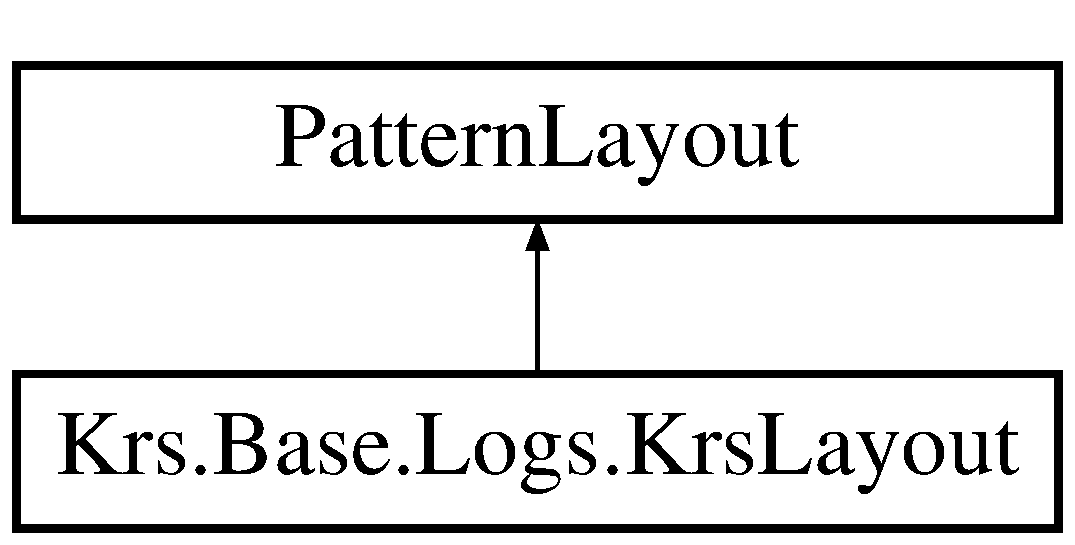
\includegraphics[height=2.000000cm]{class_krs_1_1_base_1_1_logs_1_1_krs_layout}
\end{center}
\end{figure}


\subsection{Detailed Description}
自定义布局,对自定义日志信息支持 



The documentation for this class was generated from the following file\-:\begin{DoxyCompactItemize}
\item 
Krs\-Layout.\-cs\end{DoxyCompactItemize}

\hypertarget{class_krs_1_1_base_1_1_logs_1_1_krs_message_pattern_converter}{\section{Krs.\-Base.\-Logs.\-Krs\-Message\-Pattern\-Converter Class Reference}
\label{class_krs_1_1_base_1_1_logs_1_1_krs_message_pattern_converter}\index{Krs.\-Base.\-Logs.\-Krs\-Message\-Pattern\-Converter@{Krs.\-Base.\-Logs.\-Krs\-Message\-Pattern\-Converter}}
}


模式转换  


Inheritance diagram for Krs.\-Base.\-Logs.\-Krs\-Message\-Pattern\-Converter\-:\begin{figure}[H]
\begin{center}
\leavevmode
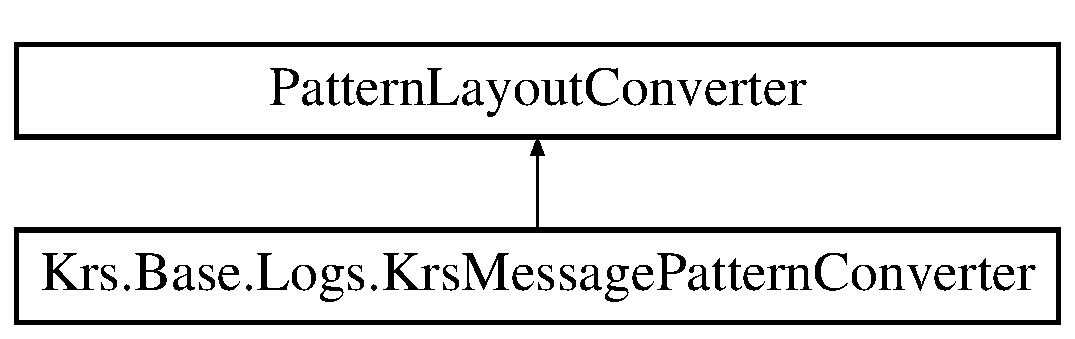
\includegraphics[height=2.000000cm]{class_krs_1_1_base_1_1_logs_1_1_krs_message_pattern_converter}
\end{center}
\end{figure}
\subsection*{Protected Member Functions}
\begin{DoxyCompactItemize}
\item 
\hypertarget{class_krs_1_1_base_1_1_logs_1_1_krs_message_pattern_converter_a17e6b4afb9ba9d5babbf7c96fdc16f58}{override void {\bfseries Convert} (System.\-I\-O.\-Text\-Writer writer, log4net.\-Core.\-Logging\-Event logging\-Event)}\label{class_krs_1_1_base_1_1_logs_1_1_krs_message_pattern_converter_a17e6b4afb9ba9d5babbf7c96fdc16f58}

\end{DoxyCompactItemize}


\subsection{Detailed Description}
模式转换 



The documentation for this class was generated from the following file\-:\begin{DoxyCompactItemize}
\item 
Krs\-Message\-Pattern\-Converter.\-cs\end{DoxyCompactItemize}

\hypertarget{class_krs_1_1_base_1_1_logs_1_1_logger}{\section{Krs.\-Base.\-Logs.\-Logger Class Reference}
\label{class_krs_1_1_base_1_1_logs_1_1_logger}\index{Krs.\-Base.\-Logs.\-Logger@{Krs.\-Base.\-Logs.\-Logger}}
}


The documentation for this class was generated from the following file\-:\begin{DoxyCompactItemize}
\item 
Logger.\-cs\end{DoxyCompactItemize}

\hypertarget{class_krs_1_1_base_1_1_logs_1_1_log_message_helper}{\section{Krs.\-Base.\-Logs.\-Log\-Message\-Helper Class Reference}
\label{class_krs_1_1_base_1_1_logs_1_1_log_message_helper}\index{Krs.\-Base.\-Logs.\-Log\-Message\-Helper@{Krs.\-Base.\-Logs.\-Log\-Message\-Helper}}
}
\subsection*{Static Public Member Functions}
\begin{DoxyCompactItemize}
\item 
static void \hyperlink{class_krs_1_1_base_1_1_logs_1_1_log_message_helper_a5197df3b485e1a2aed43c6c631912b37}{Log\-D\-E\-B\-U\-G} (string msg, string log\-Class, string sub\-Class, Dictionary$<$ string, string $>$ pars, Dictionary$<$ string, string $>$ results, Exception ex)
\begin{DoxyCompactList}\small\item\em 写入\-D\-E\-B\-U\-G日志 \end{DoxyCompactList}\item 
static void \hyperlink{class_krs_1_1_base_1_1_logs_1_1_log_message_helper_a6e00fa84c7a3101618f5ea2224dd2bbe}{Log\-I\-N\-F\-O} (string msg, string log\-Class, string sub\-Class, Dictionary$<$ string, string $>$ pars, Dictionary$<$ string, string $>$ results, Exception ex)
\begin{DoxyCompactList}\small\item\em 写入\-I\-N\-F\-O日志 \end{DoxyCompactList}\item 
static void \hyperlink{class_krs_1_1_base_1_1_logs_1_1_log_message_helper_a6ec7fedb53dc620e15c12b9e4cbdfb5f}{Log\-E\-R\-R\-O\-R} (string msg, string log\-Class, string sub\-Class, Dictionary$<$ string, string $>$ pars, Dictionary$<$ string, string $>$ results, Exception ex)
\begin{DoxyCompactList}\small\item\em 写入\-E\-R\-R\-O\-R日志 \end{DoxyCompactList}\item 
static void \hyperlink{class_krs_1_1_base_1_1_logs_1_1_log_message_helper_ab0482eaac7f87a7a0f1e9e8297ede3e4}{Log\-D\-E\-B\-U\-G} (string msg, string log\-Class, string sub\-Class, Dictionary$<$ string, object $>$ pars, Dictionary$<$ string, object $>$ results, Exception ex)
\begin{DoxyCompactList}\small\item\em 写入\-D\-E\-B\-U\-G日志 \end{DoxyCompactList}\item 
static void \hyperlink{class_krs_1_1_base_1_1_logs_1_1_log_message_helper_abc4e2ce94da5039126ee3cef5f400e45}{Log\-I\-N\-F\-O} (string msg, string log\-Class, string sub\-Class, Dictionary$<$ string, object $>$ pars, Dictionary$<$ string, object $>$ results, Exception ex)
\begin{DoxyCompactList}\small\item\em 写入\-I\-N\-F\-O日志 \end{DoxyCompactList}\item 
static void \hyperlink{class_krs_1_1_base_1_1_logs_1_1_log_message_helper_aa99965abc19b71839ad84270b840f798}{Log\-E\-R\-R\-O\-R} (string msg, string log\-Class, string sub\-Class, Dictionary$<$ string, object $>$ pars, Dictionary$<$ string, object $>$ results, Exception ex)
\begin{DoxyCompactList}\small\item\em 写入\-E\-R\-R\-O\-R日志 \end{DoxyCompactList}\item 
static void \hyperlink{class_krs_1_1_base_1_1_logs_1_1_log_message_helper_af054faa7b1cd9331f13456582a290a43}{Log\-D\-E\-B\-U\-G} (string msg, string log\-Class, string sub\-Class, Dictionary$<$ string, string $>$ pars, Dictionary$<$ string, string $>$ results)
\begin{DoxyCompactList}\small\item\em 写入\-D\-E\-B\-U\-G日志 \end{DoxyCompactList}\item 
static void \hyperlink{class_krs_1_1_base_1_1_logs_1_1_log_message_helper_aa48801ce0e7b2ac3d5b1622c4552c2b6}{Log\-I\-N\-F\-O} (string msg, string log\-Class, string sub\-Class, Dictionary$<$ string, string $>$ pars, Dictionary$<$ string, string $>$ results)
\begin{DoxyCompactList}\small\item\em 写入\-I\-N\-F\-O日志 \end{DoxyCompactList}\item 
static void \hyperlink{class_krs_1_1_base_1_1_logs_1_1_log_message_helper_acb69e510fe7d23c3f916e7bf625f72b1}{Log\-E\-R\-R\-O\-R} (string msg, string log\-Class, string sub\-Class, Dictionary$<$ string, string $>$ pars, Dictionary$<$ string, string $>$ results)
\begin{DoxyCompactList}\small\item\em 写入\-E\-R\-R\-O\-R日志 \end{DoxyCompactList}\item 
static void \hyperlink{class_krs_1_1_base_1_1_logs_1_1_log_message_helper_a49ab5d82764bd919a223642892cbc512}{Log\-D\-E\-B\-U\-G} (string msg, Dictionary$<$ string, string $>$ pars, Dictionary$<$ string, string $>$ results, Exception ex)
\begin{DoxyCompactList}\small\item\em 写入\-D\-E\-B\-U\-G日志 \end{DoxyCompactList}\item 
static void \hyperlink{class_krs_1_1_base_1_1_logs_1_1_log_message_helper_af4ec7527336b0786088dfd9f6c9eb10e}{Log\-I\-N\-F\-O} (string msg, Dictionary$<$ string, string $>$ pars, Dictionary$<$ string, string $>$ results, Exception ex)
\begin{DoxyCompactList}\small\item\em 写入\-I\-N\-F\-O日志 \end{DoxyCompactList}\item 
static void \hyperlink{class_krs_1_1_base_1_1_logs_1_1_log_message_helper_abf49053fbeeb35ade54a8f37528d5ecb}{Log\-E\-R\-R\-O\-R} (string msg, Dictionary$<$ string, string $>$ pars, Dictionary$<$ string, string $>$ results, Exception ex)
\begin{DoxyCompactList}\small\item\em 写入\-E\-R\-R\-O\-R日志 \end{DoxyCompactList}\item 
static void \hyperlink{class_krs_1_1_base_1_1_logs_1_1_log_message_helper_a9cd078d57f34d3168acd31f9cdb82787}{Log\-D\-E\-B\-U\-G} (string msg)
\begin{DoxyCompactList}\small\item\em 写入\-D\-E\-B\-U\-G日志 \end{DoxyCompactList}\item 
static void \hyperlink{class_krs_1_1_base_1_1_logs_1_1_log_message_helper_a48887a81a432460cf5a0af40d29bd0ef}{Log\-I\-N\-F\-O} (string msg)
\begin{DoxyCompactList}\small\item\em 写入\-I\-N\-F\-O日志 \end{DoxyCompactList}\item 
static void \hyperlink{class_krs_1_1_base_1_1_logs_1_1_log_message_helper_ac5f47a6b0eff7848ce0317cf6ef36e15}{Log\-E\-R\-R\-O\-R} (string msg)
\begin{DoxyCompactList}\small\item\em 写入\-E\-R\-R\-O\-R日志 \end{DoxyCompactList}\item 
static void \hyperlink{class_krs_1_1_base_1_1_logs_1_1_log_message_helper_a16cb3e63f48ad5e9ed2a6bc523439383}{Log\-D\-E\-B\-U\-G} (string msg, Exception ex)
\begin{DoxyCompactList}\small\item\em 写入\-D\-E\-B\-U\-G日志 \end{DoxyCompactList}\item 
static void \hyperlink{class_krs_1_1_base_1_1_logs_1_1_log_message_helper_aa2b82218ce5727b09bef28a5d2a38a36}{Log\-I\-N\-F\-O} (string msg, Exception ex)
\begin{DoxyCompactList}\small\item\em 写入\-I\-N\-F\-O日志 \end{DoxyCompactList}\item 
static void \hyperlink{class_krs_1_1_base_1_1_logs_1_1_log_message_helper_ab4e1ef6082f482e420289345d371c2f0}{Log\-E\-R\-R\-O\-R} (string msg, Exception ex)
\begin{DoxyCompactList}\small\item\em 写入\-E\-R\-R\-O\-R日志 \end{DoxyCompactList}\item 
static void \hyperlink{class_krs_1_1_base_1_1_logs_1_1_log_message_helper_a142af08f04810239e0ecbb58fa4860df}{Log\-D\-E\-B\-U\-G} (string msg, Dictionary$<$ string, string $>$ pars, Dictionary$<$ string, string $>$ results)
\begin{DoxyCompactList}\small\item\em 写入\-D\-E\-B\-U\-G日志 \end{DoxyCompactList}\item 
static void \hyperlink{class_krs_1_1_base_1_1_logs_1_1_log_message_helper_a38f1dc7fbff4458852982bbeb2578d7a}{Log\-I\-N\-F\-O} (string msg, Dictionary$<$ string, string $>$ pars, Dictionary$<$ string, string $>$ results)
\begin{DoxyCompactList}\small\item\em 写入\-I\-N\-F\-O日志 \end{DoxyCompactList}\item 
static void \hyperlink{class_krs_1_1_base_1_1_logs_1_1_log_message_helper_ae29b0fc865b54c4faa7c4c3de941a2ce}{Log\-E\-R\-R\-O\-R} (string msg, Dictionary$<$ string, string $>$ pars, Dictionary$<$ string, string $>$ results)
\begin{DoxyCompactList}\small\item\em 写入\-E\-R\-R\-O\-R日志 \end{DoxyCompactList}\item 
static void \hyperlink{class_krs_1_1_base_1_1_logs_1_1_log_message_helper_a54844348ebfe09eb652b1647fc5323b4}{Log\-D\-E\-B\-U\-G} (string msg, string log\-Class, string sub\-Class, Exception ex)
\begin{DoxyCompactList}\small\item\em 写入\-D\-E\-B\-U\-G日志 \end{DoxyCompactList}\item 
static void \hyperlink{class_krs_1_1_base_1_1_logs_1_1_log_message_helper_a33d1ece2923b5cc5a9ad1e931391aac4}{Log\-I\-N\-F\-O} (string msg, string log\-Class, string sub\-Class, Exception ex)
\begin{DoxyCompactList}\small\item\em 写入\-I\-N\-F\-O日志 \end{DoxyCompactList}\item 
static void \hyperlink{class_krs_1_1_base_1_1_logs_1_1_log_message_helper_aa11832cdfa43493c5a990a9011921216}{Log\-E\-R\-R\-O\-R} (string msg, string log\-Class, string sub\-Class, Exception ex)
\begin{DoxyCompactList}\small\item\em 写入\-E\-R\-R\-O\-R日志 \end{DoxyCompactList}\end{DoxyCompactItemize}


\subsection{Member Function Documentation}
\hypertarget{class_krs_1_1_base_1_1_logs_1_1_log_message_helper_a5197df3b485e1a2aed43c6c631912b37}{\index{Krs\-::\-Base\-::\-Logs\-::\-Log\-Message\-Helper@{Krs\-::\-Base\-::\-Logs\-::\-Log\-Message\-Helper}!Log\-D\-E\-B\-U\-G@{Log\-D\-E\-B\-U\-G}}
\index{Log\-D\-E\-B\-U\-G@{Log\-D\-E\-B\-U\-G}!Krs::Base::Logs::LogMessageHelper@{Krs\-::\-Base\-::\-Logs\-::\-Log\-Message\-Helper}}
\subsubsection[{Log\-D\-E\-B\-U\-G}]{\setlength{\rightskip}{0pt plus 5cm}static void Krs.\-Base.\-Logs.\-Log\-Message\-Helper.\-Log\-D\-E\-B\-U\-G (
\begin{DoxyParamCaption}
\item[{string}]{msg, }
\item[{string}]{log\-Class, }
\item[{string}]{sub\-Class, }
\item[{Dictionary$<$ string, string $>$}]{pars, }
\item[{Dictionary$<$ string, string $>$}]{results, }
\item[{Exception}]{ex}
\end{DoxyParamCaption}
)\hspace{0.3cm}{\ttfamily [inline]}, {\ttfamily [static]}}}\label{class_krs_1_1_base_1_1_logs_1_1_log_message_helper_a5197df3b485e1a2aed43c6c631912b37}


写入\-D\-E\-B\-U\-G日志 


\begin{DoxyParams}{Parameters}
{\em out\-Style} & 日志输出类型 File\-Log或\-Data\-Base\-Log\\
\hline
{\em msg} & 日志的描述信息(不能为null)\\
\hline
{\em log\-Class} & 日志大类描述(可以为null)\\
\hline
{\em sub\-Class} & 日志小类描述(可以为null)\\
\hline
{\em pars} & 参数信息列表(可以为null)\\
\hline
{\em results} & 返回值信息列表(可以为null)\\
\hline
{\em ex} & 异常信息(可以为null)\\
\hline
\end{DoxyParams}
\hypertarget{class_krs_1_1_base_1_1_logs_1_1_log_message_helper_ab0482eaac7f87a7a0f1e9e8297ede3e4}{\index{Krs\-::\-Base\-::\-Logs\-::\-Log\-Message\-Helper@{Krs\-::\-Base\-::\-Logs\-::\-Log\-Message\-Helper}!Log\-D\-E\-B\-U\-G@{Log\-D\-E\-B\-U\-G}}
\index{Log\-D\-E\-B\-U\-G@{Log\-D\-E\-B\-U\-G}!Krs::Base::Logs::LogMessageHelper@{Krs\-::\-Base\-::\-Logs\-::\-Log\-Message\-Helper}}
\subsubsection[{Log\-D\-E\-B\-U\-G}]{\setlength{\rightskip}{0pt plus 5cm}static void Krs.\-Base.\-Logs.\-Log\-Message\-Helper.\-Log\-D\-E\-B\-U\-G (
\begin{DoxyParamCaption}
\item[{string}]{msg, }
\item[{string}]{log\-Class, }
\item[{string}]{sub\-Class, }
\item[{Dictionary$<$ string, object $>$}]{pars, }
\item[{Dictionary$<$ string, object $>$}]{results, }
\item[{Exception}]{ex}
\end{DoxyParamCaption}
)\hspace{0.3cm}{\ttfamily [inline]}, {\ttfamily [static]}}}\label{class_krs_1_1_base_1_1_logs_1_1_log_message_helper_ab0482eaac7f87a7a0f1e9e8297ede3e4}


写入\-D\-E\-B\-U\-G日志 


\begin{DoxyParams}{Parameters}
{\em out\-Style} & 日志输出类型 File\-Log或\-Data\-Base\-Log\\
\hline
{\em msg} & 日志的描述信息(不能为null)\\
\hline
{\em log\-Class} & 日志大类描述(可以为null)\\
\hline
{\em sub\-Class} & 日志小类描述(可以为null)\\
\hline
{\em pars} & 参数信息列表(可以为null)\\
\hline
{\em results} & 返回值信息列表(可以为null)\\
\hline
{\em ex} & 异常信息(可以为null)\\
\hline
\end{DoxyParams}
\hypertarget{class_krs_1_1_base_1_1_logs_1_1_log_message_helper_af054faa7b1cd9331f13456582a290a43}{\index{Krs\-::\-Base\-::\-Logs\-::\-Log\-Message\-Helper@{Krs\-::\-Base\-::\-Logs\-::\-Log\-Message\-Helper}!Log\-D\-E\-B\-U\-G@{Log\-D\-E\-B\-U\-G}}
\index{Log\-D\-E\-B\-U\-G@{Log\-D\-E\-B\-U\-G}!Krs::Base::Logs::LogMessageHelper@{Krs\-::\-Base\-::\-Logs\-::\-Log\-Message\-Helper}}
\subsubsection[{Log\-D\-E\-B\-U\-G}]{\setlength{\rightskip}{0pt plus 5cm}static void Krs.\-Base.\-Logs.\-Log\-Message\-Helper.\-Log\-D\-E\-B\-U\-G (
\begin{DoxyParamCaption}
\item[{string}]{msg, }
\item[{string}]{log\-Class, }
\item[{string}]{sub\-Class, }
\item[{Dictionary$<$ string, string $>$}]{pars, }
\item[{Dictionary$<$ string, string $>$}]{results}
\end{DoxyParamCaption}
)\hspace{0.3cm}{\ttfamily [inline]}, {\ttfamily [static]}}}\label{class_krs_1_1_base_1_1_logs_1_1_log_message_helper_af054faa7b1cd9331f13456582a290a43}


写入\-D\-E\-B\-U\-G日志 


\begin{DoxyParams}{Parameters}
{\em out\-Style} & 日志输出类型 File\-Log或\-Data\-Base\-Log\\
\hline
{\em msg} & 日志的描述信息\\
\hline
{\em log\-Class} & 日志大类描述\\
\hline
{\em sub\-Class} & 日志小类描述\\
\hline
{\em pars} & 参数信息列表\\
\hline
{\em results} & 返回值信息列表\\
\hline
\end{DoxyParams}
\hypertarget{class_krs_1_1_base_1_1_logs_1_1_log_message_helper_a49ab5d82764bd919a223642892cbc512}{\index{Krs\-::\-Base\-::\-Logs\-::\-Log\-Message\-Helper@{Krs\-::\-Base\-::\-Logs\-::\-Log\-Message\-Helper}!Log\-D\-E\-B\-U\-G@{Log\-D\-E\-B\-U\-G}}
\index{Log\-D\-E\-B\-U\-G@{Log\-D\-E\-B\-U\-G}!Krs::Base::Logs::LogMessageHelper@{Krs\-::\-Base\-::\-Logs\-::\-Log\-Message\-Helper}}
\subsubsection[{Log\-D\-E\-B\-U\-G}]{\setlength{\rightskip}{0pt plus 5cm}static void Krs.\-Base.\-Logs.\-Log\-Message\-Helper.\-Log\-D\-E\-B\-U\-G (
\begin{DoxyParamCaption}
\item[{string}]{msg, }
\item[{Dictionary$<$ string, string $>$}]{pars, }
\item[{Dictionary$<$ string, string $>$}]{results, }
\item[{Exception}]{ex}
\end{DoxyParamCaption}
)\hspace{0.3cm}{\ttfamily [inline]}, {\ttfamily [static]}}}\label{class_krs_1_1_base_1_1_logs_1_1_log_message_helper_a49ab5d82764bd919a223642892cbc512}


写入\-D\-E\-B\-U\-G日志 


\begin{DoxyParams}{Parameters}
{\em out\-Style} & 日志输出类型 File\-Log或\-Data\-Base\-Log\\
\hline
{\em msg} & 日志的描述信息\\
\hline
{\em pars} & 参数信息列表\\
\hline
{\em results} & 返回值信息列表\\
\hline
{\em ex} & 异常信息\\
\hline
\end{DoxyParams}
\hypertarget{class_krs_1_1_base_1_1_logs_1_1_log_message_helper_a9cd078d57f34d3168acd31f9cdb82787}{\index{Krs\-::\-Base\-::\-Logs\-::\-Log\-Message\-Helper@{Krs\-::\-Base\-::\-Logs\-::\-Log\-Message\-Helper}!Log\-D\-E\-B\-U\-G@{Log\-D\-E\-B\-U\-G}}
\index{Log\-D\-E\-B\-U\-G@{Log\-D\-E\-B\-U\-G}!Krs::Base::Logs::LogMessageHelper@{Krs\-::\-Base\-::\-Logs\-::\-Log\-Message\-Helper}}
\subsubsection[{Log\-D\-E\-B\-U\-G}]{\setlength{\rightskip}{0pt plus 5cm}static void Krs.\-Base.\-Logs.\-Log\-Message\-Helper.\-Log\-D\-E\-B\-U\-G (
\begin{DoxyParamCaption}
\item[{string}]{msg}
\end{DoxyParamCaption}
)\hspace{0.3cm}{\ttfamily [inline]}, {\ttfamily [static]}}}\label{class_krs_1_1_base_1_1_logs_1_1_log_message_helper_a9cd078d57f34d3168acd31f9cdb82787}


写入\-D\-E\-B\-U\-G日志 


\begin{DoxyParams}{Parameters}
{\em msg} & 日志的描述信息\\
\hline
\end{DoxyParams}
\hypertarget{class_krs_1_1_base_1_1_logs_1_1_log_message_helper_a16cb3e63f48ad5e9ed2a6bc523439383}{\index{Krs\-::\-Base\-::\-Logs\-::\-Log\-Message\-Helper@{Krs\-::\-Base\-::\-Logs\-::\-Log\-Message\-Helper}!Log\-D\-E\-B\-U\-G@{Log\-D\-E\-B\-U\-G}}
\index{Log\-D\-E\-B\-U\-G@{Log\-D\-E\-B\-U\-G}!Krs::Base::Logs::LogMessageHelper@{Krs\-::\-Base\-::\-Logs\-::\-Log\-Message\-Helper}}
\subsubsection[{Log\-D\-E\-B\-U\-G}]{\setlength{\rightskip}{0pt plus 5cm}static void Krs.\-Base.\-Logs.\-Log\-Message\-Helper.\-Log\-D\-E\-B\-U\-G (
\begin{DoxyParamCaption}
\item[{string}]{msg, }
\item[{Exception}]{ex}
\end{DoxyParamCaption}
)\hspace{0.3cm}{\ttfamily [inline]}, {\ttfamily [static]}}}\label{class_krs_1_1_base_1_1_logs_1_1_log_message_helper_a16cb3e63f48ad5e9ed2a6bc523439383}


写入\-D\-E\-B\-U\-G日志 


\begin{DoxyParams}{Parameters}
{\em msg} & 日志的描述信息\\
\hline
\end{DoxyParams}
\hypertarget{class_krs_1_1_base_1_1_logs_1_1_log_message_helper_a142af08f04810239e0ecbb58fa4860df}{\index{Krs\-::\-Base\-::\-Logs\-::\-Log\-Message\-Helper@{Krs\-::\-Base\-::\-Logs\-::\-Log\-Message\-Helper}!Log\-D\-E\-B\-U\-G@{Log\-D\-E\-B\-U\-G}}
\index{Log\-D\-E\-B\-U\-G@{Log\-D\-E\-B\-U\-G}!Krs::Base::Logs::LogMessageHelper@{Krs\-::\-Base\-::\-Logs\-::\-Log\-Message\-Helper}}
\subsubsection[{Log\-D\-E\-B\-U\-G}]{\setlength{\rightskip}{0pt plus 5cm}static void Krs.\-Base.\-Logs.\-Log\-Message\-Helper.\-Log\-D\-E\-B\-U\-G (
\begin{DoxyParamCaption}
\item[{string}]{msg, }
\item[{Dictionary$<$ string, string $>$}]{pars, }
\item[{Dictionary$<$ string, string $>$}]{results}
\end{DoxyParamCaption}
)\hspace{0.3cm}{\ttfamily [inline]}, {\ttfamily [static]}}}\label{class_krs_1_1_base_1_1_logs_1_1_log_message_helper_a142af08f04810239e0ecbb58fa4860df}


写入\-D\-E\-B\-U\-G日志 


\begin{DoxyParams}{Parameters}
{\em msg} & 日志的描述信息(不能为null)\\
\hline
{\em log\-Class} & 日志大类描述(可以为null)\\
\hline
{\em sub\-Class} & 日志小类描述(可以为null)\\
\hline
{\em pars} & 参数信息列表(可以为null)\\
\hline
{\em results} & 返回值信息列表(可以为null)\\
\hline
{\em ex} & 异常信息(可以为null)\\
\hline
\end{DoxyParams}
\hypertarget{class_krs_1_1_base_1_1_logs_1_1_log_message_helper_a54844348ebfe09eb652b1647fc5323b4}{\index{Krs\-::\-Base\-::\-Logs\-::\-Log\-Message\-Helper@{Krs\-::\-Base\-::\-Logs\-::\-Log\-Message\-Helper}!Log\-D\-E\-B\-U\-G@{Log\-D\-E\-B\-U\-G}}
\index{Log\-D\-E\-B\-U\-G@{Log\-D\-E\-B\-U\-G}!Krs::Base::Logs::LogMessageHelper@{Krs\-::\-Base\-::\-Logs\-::\-Log\-Message\-Helper}}
\subsubsection[{Log\-D\-E\-B\-U\-G}]{\setlength{\rightskip}{0pt plus 5cm}static void Krs.\-Base.\-Logs.\-Log\-Message\-Helper.\-Log\-D\-E\-B\-U\-G (
\begin{DoxyParamCaption}
\item[{string}]{msg, }
\item[{string}]{log\-Class, }
\item[{string}]{sub\-Class, }
\item[{Exception}]{ex}
\end{DoxyParamCaption}
)\hspace{0.3cm}{\ttfamily [inline]}, {\ttfamily [static]}}}\label{class_krs_1_1_base_1_1_logs_1_1_log_message_helper_a54844348ebfe09eb652b1647fc5323b4}


写入\-D\-E\-B\-U\-G日志 


\begin{DoxyParams}{Parameters}
{\em out\-Style} & 日志输出类型 File\-Log或\-Data\-Base\-Log\\
\hline
{\em msg} & 日志的描述信息(不能为null)\\
\hline
{\em log\-Class} & 日志大类描述(可以为null)\\
\hline
{\em sub\-Class} & 日志小类描述(可以为null)\\
\hline
{\em ex} & 异常信息(可以为null)\\
\hline
\end{DoxyParams}
\hypertarget{class_krs_1_1_base_1_1_logs_1_1_log_message_helper_a6ec7fedb53dc620e15c12b9e4cbdfb5f}{\index{Krs\-::\-Base\-::\-Logs\-::\-Log\-Message\-Helper@{Krs\-::\-Base\-::\-Logs\-::\-Log\-Message\-Helper}!Log\-E\-R\-R\-O\-R@{Log\-E\-R\-R\-O\-R}}
\index{Log\-E\-R\-R\-O\-R@{Log\-E\-R\-R\-O\-R}!Krs::Base::Logs::LogMessageHelper@{Krs\-::\-Base\-::\-Logs\-::\-Log\-Message\-Helper}}
\subsubsection[{Log\-E\-R\-R\-O\-R}]{\setlength{\rightskip}{0pt plus 5cm}static void Krs.\-Base.\-Logs.\-Log\-Message\-Helper.\-Log\-E\-R\-R\-O\-R (
\begin{DoxyParamCaption}
\item[{string}]{msg, }
\item[{string}]{log\-Class, }
\item[{string}]{sub\-Class, }
\item[{Dictionary$<$ string, string $>$}]{pars, }
\item[{Dictionary$<$ string, string $>$}]{results, }
\item[{Exception}]{ex}
\end{DoxyParamCaption}
)\hspace{0.3cm}{\ttfamily [inline]}, {\ttfamily [static]}}}\label{class_krs_1_1_base_1_1_logs_1_1_log_message_helper_a6ec7fedb53dc620e15c12b9e4cbdfb5f}


写入\-E\-R\-R\-O\-R日志 


\begin{DoxyParams}{Parameters}
{\em out\-Style} & 日志输出类型 File\-Log或\-Data\-Base\-Log\\
\hline
{\em msg} & 日志的描述信息(不能为null)\\
\hline
{\em log\-Class} & 日志大类描述(可以为null)\\
\hline
{\em sub\-Class} & 日志小类描述(可以为null)\\
\hline
{\em pars} & 参数信息列表(可以为null)\\
\hline
{\em results} & 返回值信息列表(可以为null)\\
\hline
{\em ex} & 异常信息(可以为null)\\
\hline
\end{DoxyParams}
\hypertarget{class_krs_1_1_base_1_1_logs_1_1_log_message_helper_aa99965abc19b71839ad84270b840f798}{\index{Krs\-::\-Base\-::\-Logs\-::\-Log\-Message\-Helper@{Krs\-::\-Base\-::\-Logs\-::\-Log\-Message\-Helper}!Log\-E\-R\-R\-O\-R@{Log\-E\-R\-R\-O\-R}}
\index{Log\-E\-R\-R\-O\-R@{Log\-E\-R\-R\-O\-R}!Krs::Base::Logs::LogMessageHelper@{Krs\-::\-Base\-::\-Logs\-::\-Log\-Message\-Helper}}
\subsubsection[{Log\-E\-R\-R\-O\-R}]{\setlength{\rightskip}{0pt plus 5cm}static void Krs.\-Base.\-Logs.\-Log\-Message\-Helper.\-Log\-E\-R\-R\-O\-R (
\begin{DoxyParamCaption}
\item[{string}]{msg, }
\item[{string}]{log\-Class, }
\item[{string}]{sub\-Class, }
\item[{Dictionary$<$ string, object $>$}]{pars, }
\item[{Dictionary$<$ string, object $>$}]{results, }
\item[{Exception}]{ex}
\end{DoxyParamCaption}
)\hspace{0.3cm}{\ttfamily [inline]}, {\ttfamily [static]}}}\label{class_krs_1_1_base_1_1_logs_1_1_log_message_helper_aa99965abc19b71839ad84270b840f798}


写入\-E\-R\-R\-O\-R日志 


\begin{DoxyParams}{Parameters}
{\em out\-Style} & 日志输出类型 File\-Log或\-Data\-Base\-Log\\
\hline
{\em msg} & 日志的描述信息(不能为null)\\
\hline
{\em log\-Class} & 日志大类描述(可以为null)\\
\hline
{\em sub\-Class} & 日志小类描述(可以为null)\\
\hline
{\em pars} & 参数信息列表(可以为null)\\
\hline
{\em results} & 返回值信息列表(可以为null)\\
\hline
{\em ex} & 异常信息(可以为null)\\
\hline
\end{DoxyParams}
\hypertarget{class_krs_1_1_base_1_1_logs_1_1_log_message_helper_acb69e510fe7d23c3f916e7bf625f72b1}{\index{Krs\-::\-Base\-::\-Logs\-::\-Log\-Message\-Helper@{Krs\-::\-Base\-::\-Logs\-::\-Log\-Message\-Helper}!Log\-E\-R\-R\-O\-R@{Log\-E\-R\-R\-O\-R}}
\index{Log\-E\-R\-R\-O\-R@{Log\-E\-R\-R\-O\-R}!Krs::Base::Logs::LogMessageHelper@{Krs\-::\-Base\-::\-Logs\-::\-Log\-Message\-Helper}}
\subsubsection[{Log\-E\-R\-R\-O\-R}]{\setlength{\rightskip}{0pt plus 5cm}static void Krs.\-Base.\-Logs.\-Log\-Message\-Helper.\-Log\-E\-R\-R\-O\-R (
\begin{DoxyParamCaption}
\item[{string}]{msg, }
\item[{string}]{log\-Class, }
\item[{string}]{sub\-Class, }
\item[{Dictionary$<$ string, string $>$}]{pars, }
\item[{Dictionary$<$ string, string $>$}]{results}
\end{DoxyParamCaption}
)\hspace{0.3cm}{\ttfamily [inline]}, {\ttfamily [static]}}}\label{class_krs_1_1_base_1_1_logs_1_1_log_message_helper_acb69e510fe7d23c3f916e7bf625f72b1}


写入\-E\-R\-R\-O\-R日志 


\begin{DoxyParams}{Parameters}
{\em out\-Style} & 日志输出类型 File\-Log或\-Data\-Base\-Log\\
\hline
{\em msg} & 日志的描述信息\\
\hline
{\em log\-Class} & 日志大类描述\\
\hline
{\em sub\-Class} & 日志小类描述\\
\hline
{\em pars} & 参数信息列表\\
\hline
{\em results} & 返回值信息列表\\
\hline
\end{DoxyParams}
\hypertarget{class_krs_1_1_base_1_1_logs_1_1_log_message_helper_abf49053fbeeb35ade54a8f37528d5ecb}{\index{Krs\-::\-Base\-::\-Logs\-::\-Log\-Message\-Helper@{Krs\-::\-Base\-::\-Logs\-::\-Log\-Message\-Helper}!Log\-E\-R\-R\-O\-R@{Log\-E\-R\-R\-O\-R}}
\index{Log\-E\-R\-R\-O\-R@{Log\-E\-R\-R\-O\-R}!Krs::Base::Logs::LogMessageHelper@{Krs\-::\-Base\-::\-Logs\-::\-Log\-Message\-Helper}}
\subsubsection[{Log\-E\-R\-R\-O\-R}]{\setlength{\rightskip}{0pt plus 5cm}static void Krs.\-Base.\-Logs.\-Log\-Message\-Helper.\-Log\-E\-R\-R\-O\-R (
\begin{DoxyParamCaption}
\item[{string}]{msg, }
\item[{Dictionary$<$ string, string $>$}]{pars, }
\item[{Dictionary$<$ string, string $>$}]{results, }
\item[{Exception}]{ex}
\end{DoxyParamCaption}
)\hspace{0.3cm}{\ttfamily [inline]}, {\ttfamily [static]}}}\label{class_krs_1_1_base_1_1_logs_1_1_log_message_helper_abf49053fbeeb35ade54a8f37528d5ecb}


写入\-E\-R\-R\-O\-R日志 


\begin{DoxyParams}{Parameters}
{\em out\-Style} & 日志输出类型 File\-Log或\-Data\-Base\-Log\\
\hline
{\em msg} & 日志的描述信息\\
\hline
{\em pars} & 参数信息列表\\
\hline
{\em results} & 返回值信息列表\\
\hline
{\em ex} & 异常信息\\
\hline
\end{DoxyParams}
\hypertarget{class_krs_1_1_base_1_1_logs_1_1_log_message_helper_ac5f47a6b0eff7848ce0317cf6ef36e15}{\index{Krs\-::\-Base\-::\-Logs\-::\-Log\-Message\-Helper@{Krs\-::\-Base\-::\-Logs\-::\-Log\-Message\-Helper}!Log\-E\-R\-R\-O\-R@{Log\-E\-R\-R\-O\-R}}
\index{Log\-E\-R\-R\-O\-R@{Log\-E\-R\-R\-O\-R}!Krs::Base::Logs::LogMessageHelper@{Krs\-::\-Base\-::\-Logs\-::\-Log\-Message\-Helper}}
\subsubsection[{Log\-E\-R\-R\-O\-R}]{\setlength{\rightskip}{0pt plus 5cm}static void Krs.\-Base.\-Logs.\-Log\-Message\-Helper.\-Log\-E\-R\-R\-O\-R (
\begin{DoxyParamCaption}
\item[{string}]{msg}
\end{DoxyParamCaption}
)\hspace{0.3cm}{\ttfamily [inline]}, {\ttfamily [static]}}}\label{class_krs_1_1_base_1_1_logs_1_1_log_message_helper_ac5f47a6b0eff7848ce0317cf6ef36e15}


写入\-E\-R\-R\-O\-R日志 


\begin{DoxyParams}{Parameters}
{\em out\-Style} & 日志输出类型 File\-Log或\-Data\-Base\-Log\\
\hline
{\em msg} & 日志的描述信息\\
\hline
{\em pars} & 参数信息列表\\
\hline
{\em results} & 返回值信息列表\\
\hline
{\em ex} & 异常信息\\
\hline
\end{DoxyParams}
\hypertarget{class_krs_1_1_base_1_1_logs_1_1_log_message_helper_ab4e1ef6082f482e420289345d371c2f0}{\index{Krs\-::\-Base\-::\-Logs\-::\-Log\-Message\-Helper@{Krs\-::\-Base\-::\-Logs\-::\-Log\-Message\-Helper}!Log\-E\-R\-R\-O\-R@{Log\-E\-R\-R\-O\-R}}
\index{Log\-E\-R\-R\-O\-R@{Log\-E\-R\-R\-O\-R}!Krs::Base::Logs::LogMessageHelper@{Krs\-::\-Base\-::\-Logs\-::\-Log\-Message\-Helper}}
\subsubsection[{Log\-E\-R\-R\-O\-R}]{\setlength{\rightskip}{0pt plus 5cm}static void Krs.\-Base.\-Logs.\-Log\-Message\-Helper.\-Log\-E\-R\-R\-O\-R (
\begin{DoxyParamCaption}
\item[{string}]{msg, }
\item[{Exception}]{ex}
\end{DoxyParamCaption}
)\hspace{0.3cm}{\ttfamily [inline]}, {\ttfamily [static]}}}\label{class_krs_1_1_base_1_1_logs_1_1_log_message_helper_ab4e1ef6082f482e420289345d371c2f0}


写入\-E\-R\-R\-O\-R日志 


\begin{DoxyParams}{Parameters}
{\em out\-Style} & 日志输出类型 File\-Log或\-Data\-Base\-Log\\
\hline
{\em msg} & 日志的描述信息\\
\hline
{\em pars} & 参数信息列表\\
\hline
{\em results} & 返回值信息列表\\
\hline
{\em ex} & 异常信息\\
\hline
\end{DoxyParams}
\hypertarget{class_krs_1_1_base_1_1_logs_1_1_log_message_helper_ae29b0fc865b54c4faa7c4c3de941a2ce}{\index{Krs\-::\-Base\-::\-Logs\-::\-Log\-Message\-Helper@{Krs\-::\-Base\-::\-Logs\-::\-Log\-Message\-Helper}!Log\-E\-R\-R\-O\-R@{Log\-E\-R\-R\-O\-R}}
\index{Log\-E\-R\-R\-O\-R@{Log\-E\-R\-R\-O\-R}!Krs::Base::Logs::LogMessageHelper@{Krs\-::\-Base\-::\-Logs\-::\-Log\-Message\-Helper}}
\subsubsection[{Log\-E\-R\-R\-O\-R}]{\setlength{\rightskip}{0pt plus 5cm}static void Krs.\-Base.\-Logs.\-Log\-Message\-Helper.\-Log\-E\-R\-R\-O\-R (
\begin{DoxyParamCaption}
\item[{string}]{msg, }
\item[{Dictionary$<$ string, string $>$}]{pars, }
\item[{Dictionary$<$ string, string $>$}]{results}
\end{DoxyParamCaption}
)\hspace{0.3cm}{\ttfamily [inline]}, {\ttfamily [static]}}}\label{class_krs_1_1_base_1_1_logs_1_1_log_message_helper_ae29b0fc865b54c4faa7c4c3de941a2ce}


写入\-E\-R\-R\-O\-R日志 


\begin{DoxyParams}{Parameters}
{\em msg} & 日志的描述信息(不能为null)\\
\hline
{\em pars} & 参数信息列表(可以为null)\\
\hline
{\em results} & 返回值信息列表(可以为null)\\
\hline
{\em ex} & 异常信息(可以为null)\\
\hline
\end{DoxyParams}
\hypertarget{class_krs_1_1_base_1_1_logs_1_1_log_message_helper_aa11832cdfa43493c5a990a9011921216}{\index{Krs\-::\-Base\-::\-Logs\-::\-Log\-Message\-Helper@{Krs\-::\-Base\-::\-Logs\-::\-Log\-Message\-Helper}!Log\-E\-R\-R\-O\-R@{Log\-E\-R\-R\-O\-R}}
\index{Log\-E\-R\-R\-O\-R@{Log\-E\-R\-R\-O\-R}!Krs::Base::Logs::LogMessageHelper@{Krs\-::\-Base\-::\-Logs\-::\-Log\-Message\-Helper}}
\subsubsection[{Log\-E\-R\-R\-O\-R}]{\setlength{\rightskip}{0pt plus 5cm}static void Krs.\-Base.\-Logs.\-Log\-Message\-Helper.\-Log\-E\-R\-R\-O\-R (
\begin{DoxyParamCaption}
\item[{string}]{msg, }
\item[{string}]{log\-Class, }
\item[{string}]{sub\-Class, }
\item[{Exception}]{ex}
\end{DoxyParamCaption}
)\hspace{0.3cm}{\ttfamily [inline]}, {\ttfamily [static]}}}\label{class_krs_1_1_base_1_1_logs_1_1_log_message_helper_aa11832cdfa43493c5a990a9011921216}


写入\-E\-R\-R\-O\-R日志 


\begin{DoxyParams}{Parameters}
{\em out\-Style} & 日志输出类型 File\-Log或\-Data\-Base\-Log\\
\hline
{\em msg} & 日志的描述信息(不能为null)\\
\hline
{\em log\-Class} & 日志大类描述(可以为null)\\
\hline
{\em sub\-Class} & 日志小类描述(可以为null)\\
\hline
{\em ex} & 异常信息(可以为null)\\
\hline
\end{DoxyParams}
\hypertarget{class_krs_1_1_base_1_1_logs_1_1_log_message_helper_a6e00fa84c7a3101618f5ea2224dd2bbe}{\index{Krs\-::\-Base\-::\-Logs\-::\-Log\-Message\-Helper@{Krs\-::\-Base\-::\-Logs\-::\-Log\-Message\-Helper}!Log\-I\-N\-F\-O@{Log\-I\-N\-F\-O}}
\index{Log\-I\-N\-F\-O@{Log\-I\-N\-F\-O}!Krs::Base::Logs::LogMessageHelper@{Krs\-::\-Base\-::\-Logs\-::\-Log\-Message\-Helper}}
\subsubsection[{Log\-I\-N\-F\-O}]{\setlength{\rightskip}{0pt plus 5cm}static void Krs.\-Base.\-Logs.\-Log\-Message\-Helper.\-Log\-I\-N\-F\-O (
\begin{DoxyParamCaption}
\item[{string}]{msg, }
\item[{string}]{log\-Class, }
\item[{string}]{sub\-Class, }
\item[{Dictionary$<$ string, string $>$}]{pars, }
\item[{Dictionary$<$ string, string $>$}]{results, }
\item[{Exception}]{ex}
\end{DoxyParamCaption}
)\hspace{0.3cm}{\ttfamily [inline]}, {\ttfamily [static]}}}\label{class_krs_1_1_base_1_1_logs_1_1_log_message_helper_a6e00fa84c7a3101618f5ea2224dd2bbe}


写入\-I\-N\-F\-O日志 


\begin{DoxyParams}{Parameters}
{\em out\-Style} & 日志输出类型 File\-Log或\-Data\-Base\-Log\\
\hline
{\em msg} & 日志的描述信息(不能为null)\\
\hline
{\em log\-Class} & 日志大类描述(可以为null)\\
\hline
{\em sub\-Class} & 日志小类描述(可以为null)\\
\hline
{\em pars} & 参数信息列表(可以为null)\\
\hline
{\em results} & 返回值信息列表(可以为null)\\
\hline
{\em ex} & 异常信息(可以为null)\\
\hline
\end{DoxyParams}
\hypertarget{class_krs_1_1_base_1_1_logs_1_1_log_message_helper_abc4e2ce94da5039126ee3cef5f400e45}{\index{Krs\-::\-Base\-::\-Logs\-::\-Log\-Message\-Helper@{Krs\-::\-Base\-::\-Logs\-::\-Log\-Message\-Helper}!Log\-I\-N\-F\-O@{Log\-I\-N\-F\-O}}
\index{Log\-I\-N\-F\-O@{Log\-I\-N\-F\-O}!Krs::Base::Logs::LogMessageHelper@{Krs\-::\-Base\-::\-Logs\-::\-Log\-Message\-Helper}}
\subsubsection[{Log\-I\-N\-F\-O}]{\setlength{\rightskip}{0pt plus 5cm}static void Krs.\-Base.\-Logs.\-Log\-Message\-Helper.\-Log\-I\-N\-F\-O (
\begin{DoxyParamCaption}
\item[{string}]{msg, }
\item[{string}]{log\-Class, }
\item[{string}]{sub\-Class, }
\item[{Dictionary$<$ string, object $>$}]{pars, }
\item[{Dictionary$<$ string, object $>$}]{results, }
\item[{Exception}]{ex}
\end{DoxyParamCaption}
)\hspace{0.3cm}{\ttfamily [inline]}, {\ttfamily [static]}}}\label{class_krs_1_1_base_1_1_logs_1_1_log_message_helper_abc4e2ce94da5039126ee3cef5f400e45}


写入\-I\-N\-F\-O日志 


\begin{DoxyParams}{Parameters}
{\em out\-Style} & 日志输出类型 File\-Log或\-Data\-Base\-Log\\
\hline
{\em msg} & 日志的描述信息(不能为null)\\
\hline
{\em log\-Class} & 日志大类描述(可以为null)\\
\hline
{\em sub\-Class} & 日志小类描述(可以为null)\\
\hline
{\em pars} & 参数信息列表(可以为null)\\
\hline
{\em results} & 返回值信息列表(可以为null)\\
\hline
{\em ex} & 异常信息(可以为null)\\
\hline
\end{DoxyParams}
\hypertarget{class_krs_1_1_base_1_1_logs_1_1_log_message_helper_aa48801ce0e7b2ac3d5b1622c4552c2b6}{\index{Krs\-::\-Base\-::\-Logs\-::\-Log\-Message\-Helper@{Krs\-::\-Base\-::\-Logs\-::\-Log\-Message\-Helper}!Log\-I\-N\-F\-O@{Log\-I\-N\-F\-O}}
\index{Log\-I\-N\-F\-O@{Log\-I\-N\-F\-O}!Krs::Base::Logs::LogMessageHelper@{Krs\-::\-Base\-::\-Logs\-::\-Log\-Message\-Helper}}
\subsubsection[{Log\-I\-N\-F\-O}]{\setlength{\rightskip}{0pt plus 5cm}static void Krs.\-Base.\-Logs.\-Log\-Message\-Helper.\-Log\-I\-N\-F\-O (
\begin{DoxyParamCaption}
\item[{string}]{msg, }
\item[{string}]{log\-Class, }
\item[{string}]{sub\-Class, }
\item[{Dictionary$<$ string, string $>$}]{pars, }
\item[{Dictionary$<$ string, string $>$}]{results}
\end{DoxyParamCaption}
)\hspace{0.3cm}{\ttfamily [inline]}, {\ttfamily [static]}}}\label{class_krs_1_1_base_1_1_logs_1_1_log_message_helper_aa48801ce0e7b2ac3d5b1622c4552c2b6}


写入\-I\-N\-F\-O日志 


\begin{DoxyParams}{Parameters}
{\em out\-Style} & 日志输出类型 File\-Log或\-Data\-Base\-Log\\
\hline
{\em msg} & 日志的描述信息\\
\hline
{\em log\-Class} & 日志大类描述\\
\hline
{\em sub\-Class} & 日志小类描述\\
\hline
{\em pars} & 参数信息列表\\
\hline
{\em results} & 返回值信息列表\\
\hline
\end{DoxyParams}
\hypertarget{class_krs_1_1_base_1_1_logs_1_1_log_message_helper_af4ec7527336b0786088dfd9f6c9eb10e}{\index{Krs\-::\-Base\-::\-Logs\-::\-Log\-Message\-Helper@{Krs\-::\-Base\-::\-Logs\-::\-Log\-Message\-Helper}!Log\-I\-N\-F\-O@{Log\-I\-N\-F\-O}}
\index{Log\-I\-N\-F\-O@{Log\-I\-N\-F\-O}!Krs::Base::Logs::LogMessageHelper@{Krs\-::\-Base\-::\-Logs\-::\-Log\-Message\-Helper}}
\subsubsection[{Log\-I\-N\-F\-O}]{\setlength{\rightskip}{0pt plus 5cm}static void Krs.\-Base.\-Logs.\-Log\-Message\-Helper.\-Log\-I\-N\-F\-O (
\begin{DoxyParamCaption}
\item[{string}]{msg, }
\item[{Dictionary$<$ string, string $>$}]{pars, }
\item[{Dictionary$<$ string, string $>$}]{results, }
\item[{Exception}]{ex}
\end{DoxyParamCaption}
)\hspace{0.3cm}{\ttfamily [inline]}, {\ttfamily [static]}}}\label{class_krs_1_1_base_1_1_logs_1_1_log_message_helper_af4ec7527336b0786088dfd9f6c9eb10e}


写入\-I\-N\-F\-O日志 


\begin{DoxyParams}{Parameters}
{\em out\-Style} & 日志输出类型 File\-Log或\-Data\-Base\-Log\\
\hline
{\em msg} & 日志的描述信息\\
\hline
{\em pars} & 参数信息列表\\
\hline
{\em results} & 返回值信息列表\\
\hline
{\em ex} & 异常信息\\
\hline
\end{DoxyParams}
\hypertarget{class_krs_1_1_base_1_1_logs_1_1_log_message_helper_a48887a81a432460cf5a0af40d29bd0ef}{\index{Krs\-::\-Base\-::\-Logs\-::\-Log\-Message\-Helper@{Krs\-::\-Base\-::\-Logs\-::\-Log\-Message\-Helper}!Log\-I\-N\-F\-O@{Log\-I\-N\-F\-O}}
\index{Log\-I\-N\-F\-O@{Log\-I\-N\-F\-O}!Krs::Base::Logs::LogMessageHelper@{Krs\-::\-Base\-::\-Logs\-::\-Log\-Message\-Helper}}
\subsubsection[{Log\-I\-N\-F\-O}]{\setlength{\rightskip}{0pt plus 5cm}static void Krs.\-Base.\-Logs.\-Log\-Message\-Helper.\-Log\-I\-N\-F\-O (
\begin{DoxyParamCaption}
\item[{string}]{msg}
\end{DoxyParamCaption}
)\hspace{0.3cm}{\ttfamily [inline]}, {\ttfamily [static]}}}\label{class_krs_1_1_base_1_1_logs_1_1_log_message_helper_a48887a81a432460cf5a0af40d29bd0ef}


写入\-I\-N\-F\-O日志 


\begin{DoxyParams}{Parameters}
{\em out\-Style} & 日志输出类型 File\-Log或\-Data\-Base\-Log\\
\hline
{\em msg} & 日志的描述信息\\
\hline
{\em pars} & 参数信息列表\\
\hline
{\em results} & 返回值信息列表\\
\hline
{\em ex} & 异常信息\\
\hline
\end{DoxyParams}
\hypertarget{class_krs_1_1_base_1_1_logs_1_1_log_message_helper_aa2b82218ce5727b09bef28a5d2a38a36}{\index{Krs\-::\-Base\-::\-Logs\-::\-Log\-Message\-Helper@{Krs\-::\-Base\-::\-Logs\-::\-Log\-Message\-Helper}!Log\-I\-N\-F\-O@{Log\-I\-N\-F\-O}}
\index{Log\-I\-N\-F\-O@{Log\-I\-N\-F\-O}!Krs::Base::Logs::LogMessageHelper@{Krs\-::\-Base\-::\-Logs\-::\-Log\-Message\-Helper}}
\subsubsection[{Log\-I\-N\-F\-O}]{\setlength{\rightskip}{0pt plus 5cm}static void Krs.\-Base.\-Logs.\-Log\-Message\-Helper.\-Log\-I\-N\-F\-O (
\begin{DoxyParamCaption}
\item[{string}]{msg, }
\item[{Exception}]{ex}
\end{DoxyParamCaption}
)\hspace{0.3cm}{\ttfamily [inline]}, {\ttfamily [static]}}}\label{class_krs_1_1_base_1_1_logs_1_1_log_message_helper_aa2b82218ce5727b09bef28a5d2a38a36}


写入\-I\-N\-F\-O日志 


\begin{DoxyParams}{Parameters}
{\em out\-Style} & 日志输出类型 File\-Log或\-Data\-Base\-Log\\
\hline
{\em msg} & 日志的描述信息\\
\hline
{\em pars} & 参数信息列表\\
\hline
{\em results} & 返回值信息列表\\
\hline
{\em ex} & 异常信息\\
\hline
\end{DoxyParams}
\hypertarget{class_krs_1_1_base_1_1_logs_1_1_log_message_helper_a38f1dc7fbff4458852982bbeb2578d7a}{\index{Krs\-::\-Base\-::\-Logs\-::\-Log\-Message\-Helper@{Krs\-::\-Base\-::\-Logs\-::\-Log\-Message\-Helper}!Log\-I\-N\-F\-O@{Log\-I\-N\-F\-O}}
\index{Log\-I\-N\-F\-O@{Log\-I\-N\-F\-O}!Krs::Base::Logs::LogMessageHelper@{Krs\-::\-Base\-::\-Logs\-::\-Log\-Message\-Helper}}
\subsubsection[{Log\-I\-N\-F\-O}]{\setlength{\rightskip}{0pt plus 5cm}static void Krs.\-Base.\-Logs.\-Log\-Message\-Helper.\-Log\-I\-N\-F\-O (
\begin{DoxyParamCaption}
\item[{string}]{msg, }
\item[{Dictionary$<$ string, string $>$}]{pars, }
\item[{Dictionary$<$ string, string $>$}]{results}
\end{DoxyParamCaption}
)\hspace{0.3cm}{\ttfamily [inline]}, {\ttfamily [static]}}}\label{class_krs_1_1_base_1_1_logs_1_1_log_message_helper_a38f1dc7fbff4458852982bbeb2578d7a}


写入\-I\-N\-F\-O日志 


\begin{DoxyParams}{Parameters}
{\em msg} & 日志的描述信息(不能为null)\\
\hline
{\em pars} & 参数信息列表(可以为null)\\
\hline
{\em results} & 返回值信息列表(可以为null)\\
\hline
{\em ex} & 异常信息(可以为null)\\
\hline
\end{DoxyParams}
\hypertarget{class_krs_1_1_base_1_1_logs_1_1_log_message_helper_a33d1ece2923b5cc5a9ad1e931391aac4}{\index{Krs\-::\-Base\-::\-Logs\-::\-Log\-Message\-Helper@{Krs\-::\-Base\-::\-Logs\-::\-Log\-Message\-Helper}!Log\-I\-N\-F\-O@{Log\-I\-N\-F\-O}}
\index{Log\-I\-N\-F\-O@{Log\-I\-N\-F\-O}!Krs::Base::Logs::LogMessageHelper@{Krs\-::\-Base\-::\-Logs\-::\-Log\-Message\-Helper}}
\subsubsection[{Log\-I\-N\-F\-O}]{\setlength{\rightskip}{0pt plus 5cm}static void Krs.\-Base.\-Logs.\-Log\-Message\-Helper.\-Log\-I\-N\-F\-O (
\begin{DoxyParamCaption}
\item[{string}]{msg, }
\item[{string}]{log\-Class, }
\item[{string}]{sub\-Class, }
\item[{Exception}]{ex}
\end{DoxyParamCaption}
)\hspace{0.3cm}{\ttfamily [inline]}, {\ttfamily [static]}}}\label{class_krs_1_1_base_1_1_logs_1_1_log_message_helper_a33d1ece2923b5cc5a9ad1e931391aac4}


写入\-I\-N\-F\-O日志 


\begin{DoxyParams}{Parameters}
{\em out\-Style} & 日志输出类型 File\-Log或\-Data\-Base\-Log\\
\hline
{\em msg} & 日志的描述信息(不能为null)\\
\hline
{\em pars} & 参数信息列表(可以为null)\\
\hline
{\em results} & 返回值信息列表(可以为null)\\
\hline
{\em ex} & 异常信息(可以为null)\\
\hline
\end{DoxyParams}


The documentation for this class was generated from the following file\-:\begin{DoxyCompactItemize}
\item 
Log\-Message\-Helper.\-cs\end{DoxyCompactItemize}

\hypertarget{class_krs_1_1_base_1_1_logs_1_1_log_message_info}{\section{Krs.\-Base.\-Logs.\-Log\-Message\-Info Class Reference}
\label{class_krs_1_1_base_1_1_logs_1_1_log_message_info}\index{Krs.\-Base.\-Logs.\-Log\-Message\-Info@{Krs.\-Base.\-Logs.\-Log\-Message\-Info}}
}


日志信息(\-Web)  


\subsection*{Static Public Member Functions}
\begin{DoxyCompactItemize}
\item 
static string \hyperlink{class_krs_1_1_base_1_1_logs_1_1_log_message_info_afbf204bbc7164a8863b15bbae78d97bb}{Get\-I\-P\-Address} ()
\begin{DoxyCompactList}\small\item\em 获取本机的\-I\-P地址 \end{DoxyCompactList}\end{DoxyCompactItemize}
\subsection*{Public Attributes}
\begin{DoxyCompactItemize}
\item 
\hypertarget{class_krs_1_1_base_1_1_logs_1_1_log_message_info_a690988c88303f2b9e568dec35abee06a}{string {\bfseries \-\_\-\-Invoke\-Desc} = string.\-Empty}\label{class_krs_1_1_base_1_1_logs_1_1_log_message_info_a690988c88303f2b9e568dec35abee06a}

\item 
\hypertarget{class_krs_1_1_base_1_1_logs_1_1_log_message_info_aec2e01758d11817fba8afdf59ada7c47}{string {\bfseries \-\_\-\-Result\-Desc} = string.\-Empty}\label{class_krs_1_1_base_1_1_logs_1_1_log_message_info_aec2e01758d11817fba8afdf59ada7c47}

\end{DoxyCompactItemize}
\subsection*{Properties}
\begin{DoxyCompactItemize}
\item 
string \hyperlink{class_krs_1_1_base_1_1_logs_1_1_log_message_info_adb1c24e24aba48719cb0cd0fbf010853}{Seq\-No}\hspace{0.3cm}{\ttfamily  \mbox{[}get\mbox{]}}
\begin{DoxyCompactList}\small\item\em 获取业务流水号 \end{DoxyCompactList}\item 
string \hyperlink{class_krs_1_1_base_1_1_logs_1_1_log_message_info_ac4632df2e0cca88fce2921fcb17f7cc4}{U\-R\-L}\hspace{0.3cm}{\ttfamily  \mbox{[}get\mbox{]}}
\begin{DoxyCompactList}\small\item\em 获取请求的\-U\-R\-L \end{DoxyCompactList}\item 
string \hyperlink{class_krs_1_1_base_1_1_logs_1_1_log_message_info_a929c7020a27daafba8b665686b35d202}{I\-P}\hspace{0.3cm}{\ttfamily  \mbox{[}get\mbox{]}}
\begin{DoxyCompactList}\small\item\em 获取客户端IP地址 \end{DoxyCompactList}\item 
string \hyperlink{class_krs_1_1_base_1_1_logs_1_1_log_message_info_a757c814599d8b9620cd075da3e9026a9}{M\-N\-G\-Code}\hspace{0.3cm}{\ttfamily  \mbox{[}get\mbox{]}}
\begin{DoxyCompactList}\small\item\em 获取或设置机构代码 \end{DoxyCompactList}\item 
string \hyperlink{class_krs_1_1_base_1_1_logs_1_1_log_message_info_a13105a83b923a9e1a27de4487eb88d3f}{App\-Flag}\hspace{0.3cm}{\ttfamily  \mbox{[}get\mbox{]}}
\begin{DoxyCompactList}\small\item\em 应用程序标识 \end{DoxyCompactList}\item 
string \hyperlink{class_krs_1_1_base_1_1_logs_1_1_log_message_info_a8fa26acb35e4aa3e7aebb41f3ad9a431}{User\-Name}\hspace{0.3cm}{\ttfamily  \mbox{[}get\mbox{]}}
\begin{DoxyCompactList}\small\item\em 获取或设置系统登陆用户(id/name) \end{DoxyCompactList}\item 
string \hyperlink{class_krs_1_1_base_1_1_logs_1_1_log_message_info_a605395da814c8a43a7cdc3831d7f51cd}{Log\-From}\hspace{0.3cm}{\ttfamily  \mbox{[}get\mbox{]}}
\begin{DoxyCompactList}\small\item\em 获取或设置系统登陆用户(id/name) \end{DoxyCompactList}\item 
\hyperlink{namespace_krs_1_1_base_1_1_logs_aa1f948e33e410052b2716d8b68ec6583}{Log\-Level} \hyperlink{class_krs_1_1_base_1_1_logs_1_1_log_message_info_a5649136dbdcee8cd457230a0a4f99e20}{Level}\hspace{0.3cm}{\ttfamily  \mbox{[}set\mbox{]}}
\begin{DoxyCompactList}\small\item\em 获取或设置日志级别(默认为info) \end{DoxyCompactList}\item 
\hypertarget{class_krs_1_1_base_1_1_logs_1_1_log_message_info_a7b249b29a84cf019de4a97e522f64f83}{string {\bfseries Level\-Log}\hspace{0.3cm}{\ttfamily  \mbox{[}get\mbox{]}}}\label{class_krs_1_1_base_1_1_logs_1_1_log_message_info_a7b249b29a84cf019de4a97e522f64f83}

\item 
string \hyperlink{class_krs_1_1_base_1_1_logs_1_1_log_message_info_a4eb05dff1f7e3559293a1140a508ead4}{Log\-Class}\hspace{0.3cm}{\ttfamily  \mbox{[}get, set\mbox{]}}
\begin{DoxyCompactList}\small\item\em 获取或设置日志分类(具体的模块名) \end{DoxyCompactList}\item 
string \hyperlink{class_krs_1_1_base_1_1_logs_1_1_log_message_info_a8bb4cfd86598b8fac3ad1d1a7cf2d24b}{Sub\-Class}\hspace{0.3cm}{\ttfamily  \mbox{[}get, set\mbox{]}}
\begin{DoxyCompactList}\small\item\em 获取或设置日志小类(全路径类或页面地址或方法名) \end{DoxyCompactList}\item 
string \hyperlink{class_krs_1_1_base_1_1_logs_1_1_log_message_info_adf3328dc8f0b7ff66f3763b5677508cb}{Call\-Desc}\hspace{0.3cm}{\ttfamily  \mbox{[}get, set\mbox{]}}
\begin{DoxyCompactList}\small\item\em 日志调用方方法的描述 \end{DoxyCompactList}\item 
string \hyperlink{class_krs_1_1_base_1_1_logs_1_1_log_message_info_afdb3e79026f50bda1d7cb31a320c915d}{Param\-Desc}\hspace{0.3cm}{\ttfamily  \mbox{[}get, set\mbox{]}}
\begin{DoxyCompactList}\small\item\em 获取或设置参数信息描述 \end{DoxyCompactList}\item 
string \hyperlink{class_krs_1_1_base_1_1_logs_1_1_log_message_info_a5f071f620e31a0e1d982b7dbd6402036}{Result\-Desc}\hspace{0.3cm}{\ttfamily  \mbox{[}get, set\mbox{]}}
\begin{DoxyCompactList}\small\item\em 获取或设置返回值信息描述 \end{DoxyCompactList}\item 
string \hyperlink{class_krs_1_1_base_1_1_logs_1_1_log_message_info_a91ae058e58f68a99ce008f375b63f805}{Details}\hspace{0.3cm}{\ttfamily  \mbox{[}get, set\mbox{]}}
\begin{DoxyCompactList}\small\item\em 获取或设置日志详细信息描述 \end{DoxyCompactList}\item 
string \hyperlink{class_krs_1_1_base_1_1_logs_1_1_log_message_info_aba5adde9a540d4b52dbaac6ebec60b16}{Error\-Msg}\hspace{0.3cm}{\ttfamily  \mbox{[}get, set\mbox{]}}
\begin{DoxyCompactList}\small\item\em 异常信息描述 \end{DoxyCompactList}\end{DoxyCompactItemize}


\subsection{Detailed Description}
日志信息(\-Web) 



\subsection{Member Function Documentation}
\hypertarget{class_krs_1_1_base_1_1_logs_1_1_log_message_info_afbf204bbc7164a8863b15bbae78d97bb}{\index{Krs\-::\-Base\-::\-Logs\-::\-Log\-Message\-Info@{Krs\-::\-Base\-::\-Logs\-::\-Log\-Message\-Info}!Get\-I\-P\-Address@{Get\-I\-P\-Address}}
\index{Get\-I\-P\-Address@{Get\-I\-P\-Address}!Krs::Base::Logs::LogMessageInfo@{Krs\-::\-Base\-::\-Logs\-::\-Log\-Message\-Info}}
\subsubsection[{Get\-I\-P\-Address}]{\setlength{\rightskip}{0pt plus 5cm}static string Krs.\-Base.\-Logs.\-Log\-Message\-Info.\-Get\-I\-P\-Address (
\begin{DoxyParamCaption}
{}
\end{DoxyParamCaption}
)\hspace{0.3cm}{\ttfamily [inline]}, {\ttfamily [static]}}}\label{class_krs_1_1_base_1_1_logs_1_1_log_message_info_afbf204bbc7164a8863b15bbae78d97bb}


获取本机的\-I\-P地址 



\subsection{Property Documentation}
\hypertarget{class_krs_1_1_base_1_1_logs_1_1_log_message_info_a13105a83b923a9e1a27de4487eb88d3f}{\index{Krs\-::\-Base\-::\-Logs\-::\-Log\-Message\-Info@{Krs\-::\-Base\-::\-Logs\-::\-Log\-Message\-Info}!App\-Flag@{App\-Flag}}
\index{App\-Flag@{App\-Flag}!Krs::Base::Logs::LogMessageInfo@{Krs\-::\-Base\-::\-Logs\-::\-Log\-Message\-Info}}
\subsubsection[{App\-Flag}]{\setlength{\rightskip}{0pt plus 5cm}string Krs.\-Base.\-Logs.\-Log\-Message\-Info.\-App\-Flag\hspace{0.3cm}{\ttfamily [get]}}}\label{class_krs_1_1_base_1_1_logs_1_1_log_message_info_a13105a83b923a9e1a27de4487eb88d3f}


应用程序标识 

\hypertarget{class_krs_1_1_base_1_1_logs_1_1_log_message_info_adf3328dc8f0b7ff66f3763b5677508cb}{\index{Krs\-::\-Base\-::\-Logs\-::\-Log\-Message\-Info@{Krs\-::\-Base\-::\-Logs\-::\-Log\-Message\-Info}!Call\-Desc@{Call\-Desc}}
\index{Call\-Desc@{Call\-Desc}!Krs::Base::Logs::LogMessageInfo@{Krs\-::\-Base\-::\-Logs\-::\-Log\-Message\-Info}}
\subsubsection[{Call\-Desc}]{\setlength{\rightskip}{0pt plus 5cm}string Krs.\-Base.\-Logs.\-Log\-Message\-Info.\-Call\-Desc\hspace{0.3cm}{\ttfamily [get]}, {\ttfamily [set]}}}\label{class_krs_1_1_base_1_1_logs_1_1_log_message_info_adf3328dc8f0b7ff66f3763b5677508cb}


日志调用方方法的描述 

\hypertarget{class_krs_1_1_base_1_1_logs_1_1_log_message_info_a91ae058e58f68a99ce008f375b63f805}{\index{Krs\-::\-Base\-::\-Logs\-::\-Log\-Message\-Info@{Krs\-::\-Base\-::\-Logs\-::\-Log\-Message\-Info}!Details@{Details}}
\index{Details@{Details}!Krs::Base::Logs::LogMessageInfo@{Krs\-::\-Base\-::\-Logs\-::\-Log\-Message\-Info}}
\subsubsection[{Details}]{\setlength{\rightskip}{0pt plus 5cm}string Krs.\-Base.\-Logs.\-Log\-Message\-Info.\-Details\hspace{0.3cm}{\ttfamily [get]}, {\ttfamily [set]}}}\label{class_krs_1_1_base_1_1_logs_1_1_log_message_info_a91ae058e58f68a99ce008f375b63f805}


获取或设置日志详细信息描述 

\hypertarget{class_krs_1_1_base_1_1_logs_1_1_log_message_info_aba5adde9a540d4b52dbaac6ebec60b16}{\index{Krs\-::\-Base\-::\-Logs\-::\-Log\-Message\-Info@{Krs\-::\-Base\-::\-Logs\-::\-Log\-Message\-Info}!Error\-Msg@{Error\-Msg}}
\index{Error\-Msg@{Error\-Msg}!Krs::Base::Logs::LogMessageInfo@{Krs\-::\-Base\-::\-Logs\-::\-Log\-Message\-Info}}
\subsubsection[{Error\-Msg}]{\setlength{\rightskip}{0pt plus 5cm}string Krs.\-Base.\-Logs.\-Log\-Message\-Info.\-Error\-Msg\hspace{0.3cm}{\ttfamily [get]}, {\ttfamily [set]}}}\label{class_krs_1_1_base_1_1_logs_1_1_log_message_info_aba5adde9a540d4b52dbaac6ebec60b16}


异常信息描述 

\hypertarget{class_krs_1_1_base_1_1_logs_1_1_log_message_info_a929c7020a27daafba8b665686b35d202}{\index{Krs\-::\-Base\-::\-Logs\-::\-Log\-Message\-Info@{Krs\-::\-Base\-::\-Logs\-::\-Log\-Message\-Info}!I\-P@{I\-P}}
\index{I\-P@{I\-P}!Krs::Base::Logs::LogMessageInfo@{Krs\-::\-Base\-::\-Logs\-::\-Log\-Message\-Info}}
\subsubsection[{I\-P}]{\setlength{\rightskip}{0pt plus 5cm}string Krs.\-Base.\-Logs.\-Log\-Message\-Info.\-I\-P\hspace{0.3cm}{\ttfamily [get]}}}\label{class_krs_1_1_base_1_1_logs_1_1_log_message_info_a929c7020a27daafba8b665686b35d202}


获取客户端IP地址 

\hypertarget{class_krs_1_1_base_1_1_logs_1_1_log_message_info_a5649136dbdcee8cd457230a0a4f99e20}{\index{Krs\-::\-Base\-::\-Logs\-::\-Log\-Message\-Info@{Krs\-::\-Base\-::\-Logs\-::\-Log\-Message\-Info}!Level@{Level}}
\index{Level@{Level}!Krs::Base::Logs::LogMessageInfo@{Krs\-::\-Base\-::\-Logs\-::\-Log\-Message\-Info}}
\subsubsection[{Level}]{\setlength{\rightskip}{0pt plus 5cm}{\bf Log\-Level} Krs.\-Base.\-Logs.\-Log\-Message\-Info.\-Level\hspace{0.3cm}{\ttfamily [set]}}}\label{class_krs_1_1_base_1_1_logs_1_1_log_message_info_a5649136dbdcee8cd457230a0a4f99e20}


获取或设置日志级别(默认为info) 

\hypertarget{class_krs_1_1_base_1_1_logs_1_1_log_message_info_a4eb05dff1f7e3559293a1140a508ead4}{\index{Krs\-::\-Base\-::\-Logs\-::\-Log\-Message\-Info@{Krs\-::\-Base\-::\-Logs\-::\-Log\-Message\-Info}!Log\-Class@{Log\-Class}}
\index{Log\-Class@{Log\-Class}!Krs::Base::Logs::LogMessageInfo@{Krs\-::\-Base\-::\-Logs\-::\-Log\-Message\-Info}}
\subsubsection[{Log\-Class}]{\setlength{\rightskip}{0pt plus 5cm}string Krs.\-Base.\-Logs.\-Log\-Message\-Info.\-Log\-Class\hspace{0.3cm}{\ttfamily [get]}, {\ttfamily [set]}}}\label{class_krs_1_1_base_1_1_logs_1_1_log_message_info_a4eb05dff1f7e3559293a1140a508ead4}


获取或设置日志分类(具体的模块名) 

\hypertarget{class_krs_1_1_base_1_1_logs_1_1_log_message_info_a605395da814c8a43a7cdc3831d7f51cd}{\index{Krs\-::\-Base\-::\-Logs\-::\-Log\-Message\-Info@{Krs\-::\-Base\-::\-Logs\-::\-Log\-Message\-Info}!Log\-From@{Log\-From}}
\index{Log\-From@{Log\-From}!Krs::Base::Logs::LogMessageInfo@{Krs\-::\-Base\-::\-Logs\-::\-Log\-Message\-Info}}
\subsubsection[{Log\-From}]{\setlength{\rightskip}{0pt plus 5cm}string Krs.\-Base.\-Logs.\-Log\-Message\-Info.\-Log\-From\hspace{0.3cm}{\ttfamily [get]}}}\label{class_krs_1_1_base_1_1_logs_1_1_log_message_info_a605395da814c8a43a7cdc3831d7f51cd}


获取或设置系统登陆用户(id/name) 

\hypertarget{class_krs_1_1_base_1_1_logs_1_1_log_message_info_a757c814599d8b9620cd075da3e9026a9}{\index{Krs\-::\-Base\-::\-Logs\-::\-Log\-Message\-Info@{Krs\-::\-Base\-::\-Logs\-::\-Log\-Message\-Info}!M\-N\-G\-Code@{M\-N\-G\-Code}}
\index{M\-N\-G\-Code@{M\-N\-G\-Code}!Krs::Base::Logs::LogMessageInfo@{Krs\-::\-Base\-::\-Logs\-::\-Log\-Message\-Info}}
\subsubsection[{M\-N\-G\-Code}]{\setlength{\rightskip}{0pt plus 5cm}string Krs.\-Base.\-Logs.\-Log\-Message\-Info.\-M\-N\-G\-Code\hspace{0.3cm}{\ttfamily [get]}}}\label{class_krs_1_1_base_1_1_logs_1_1_log_message_info_a757c814599d8b9620cd075da3e9026a9}


获取或设置机构代码 

\hypertarget{class_krs_1_1_base_1_1_logs_1_1_log_message_info_afdb3e79026f50bda1d7cb31a320c915d}{\index{Krs\-::\-Base\-::\-Logs\-::\-Log\-Message\-Info@{Krs\-::\-Base\-::\-Logs\-::\-Log\-Message\-Info}!Param\-Desc@{Param\-Desc}}
\index{Param\-Desc@{Param\-Desc}!Krs::Base::Logs::LogMessageInfo@{Krs\-::\-Base\-::\-Logs\-::\-Log\-Message\-Info}}
\subsubsection[{Param\-Desc}]{\setlength{\rightskip}{0pt plus 5cm}string Krs.\-Base.\-Logs.\-Log\-Message\-Info.\-Param\-Desc\hspace{0.3cm}{\ttfamily [get]}, {\ttfamily [set]}}}\label{class_krs_1_1_base_1_1_logs_1_1_log_message_info_afdb3e79026f50bda1d7cb31a320c915d}


获取或设置参数信息描述 

\hypertarget{class_krs_1_1_base_1_1_logs_1_1_log_message_info_a5f071f620e31a0e1d982b7dbd6402036}{\index{Krs\-::\-Base\-::\-Logs\-::\-Log\-Message\-Info@{Krs\-::\-Base\-::\-Logs\-::\-Log\-Message\-Info}!Result\-Desc@{Result\-Desc}}
\index{Result\-Desc@{Result\-Desc}!Krs::Base::Logs::LogMessageInfo@{Krs\-::\-Base\-::\-Logs\-::\-Log\-Message\-Info}}
\subsubsection[{Result\-Desc}]{\setlength{\rightskip}{0pt plus 5cm}string Krs.\-Base.\-Logs.\-Log\-Message\-Info.\-Result\-Desc\hspace{0.3cm}{\ttfamily [get]}, {\ttfamily [set]}}}\label{class_krs_1_1_base_1_1_logs_1_1_log_message_info_a5f071f620e31a0e1d982b7dbd6402036}


获取或设置返回值信息描述 

\hypertarget{class_krs_1_1_base_1_1_logs_1_1_log_message_info_adb1c24e24aba48719cb0cd0fbf010853}{\index{Krs\-::\-Base\-::\-Logs\-::\-Log\-Message\-Info@{Krs\-::\-Base\-::\-Logs\-::\-Log\-Message\-Info}!Seq\-No@{Seq\-No}}
\index{Seq\-No@{Seq\-No}!Krs::Base::Logs::LogMessageInfo@{Krs\-::\-Base\-::\-Logs\-::\-Log\-Message\-Info}}
\subsubsection[{Seq\-No}]{\setlength{\rightskip}{0pt plus 5cm}string Krs.\-Base.\-Logs.\-Log\-Message\-Info.\-Seq\-No\hspace{0.3cm}{\ttfamily [get]}}}\label{class_krs_1_1_base_1_1_logs_1_1_log_message_info_adb1c24e24aba48719cb0cd0fbf010853}


获取业务流水号 

\hypertarget{class_krs_1_1_base_1_1_logs_1_1_log_message_info_a8bb4cfd86598b8fac3ad1d1a7cf2d24b}{\index{Krs\-::\-Base\-::\-Logs\-::\-Log\-Message\-Info@{Krs\-::\-Base\-::\-Logs\-::\-Log\-Message\-Info}!Sub\-Class@{Sub\-Class}}
\index{Sub\-Class@{Sub\-Class}!Krs::Base::Logs::LogMessageInfo@{Krs\-::\-Base\-::\-Logs\-::\-Log\-Message\-Info}}
\subsubsection[{Sub\-Class}]{\setlength{\rightskip}{0pt plus 5cm}string Krs.\-Base.\-Logs.\-Log\-Message\-Info.\-Sub\-Class\hspace{0.3cm}{\ttfamily [get]}, {\ttfamily [set]}}}\label{class_krs_1_1_base_1_1_logs_1_1_log_message_info_a8bb4cfd86598b8fac3ad1d1a7cf2d24b}


获取或设置日志小类(全路径类或页面地址或方法名) 

\hypertarget{class_krs_1_1_base_1_1_logs_1_1_log_message_info_ac4632df2e0cca88fce2921fcb17f7cc4}{\index{Krs\-::\-Base\-::\-Logs\-::\-Log\-Message\-Info@{Krs\-::\-Base\-::\-Logs\-::\-Log\-Message\-Info}!U\-R\-L@{U\-R\-L}}
\index{U\-R\-L@{U\-R\-L}!Krs::Base::Logs::LogMessageInfo@{Krs\-::\-Base\-::\-Logs\-::\-Log\-Message\-Info}}
\subsubsection[{U\-R\-L}]{\setlength{\rightskip}{0pt plus 5cm}string Krs.\-Base.\-Logs.\-Log\-Message\-Info.\-U\-R\-L\hspace{0.3cm}{\ttfamily [get]}}}\label{class_krs_1_1_base_1_1_logs_1_1_log_message_info_ac4632df2e0cca88fce2921fcb17f7cc4}


获取请求的\-U\-R\-L 

\hypertarget{class_krs_1_1_base_1_1_logs_1_1_log_message_info_a8fa26acb35e4aa3e7aebb41f3ad9a431}{\index{Krs\-::\-Base\-::\-Logs\-::\-Log\-Message\-Info@{Krs\-::\-Base\-::\-Logs\-::\-Log\-Message\-Info}!User\-Name@{User\-Name}}
\index{User\-Name@{User\-Name}!Krs::Base::Logs::LogMessageInfo@{Krs\-::\-Base\-::\-Logs\-::\-Log\-Message\-Info}}
\subsubsection[{User\-Name}]{\setlength{\rightskip}{0pt plus 5cm}string Krs.\-Base.\-Logs.\-Log\-Message\-Info.\-User\-Name\hspace{0.3cm}{\ttfamily [get]}}}\label{class_krs_1_1_base_1_1_logs_1_1_log_message_info_a8fa26acb35e4aa3e7aebb41f3ad9a431}


获取或设置系统登陆用户(id/name) 



The documentation for this class was generated from the following file\-:\begin{DoxyCompactItemize}
\item 
Log\-Message\-Info.\-cs\end{DoxyCompactItemize}

\hypertarget{class_krs_1_1_base_1_1_logs_1_1_run_time_loger}{\section{Krs.\-Base.\-Logs.\-Run\-Time\-Loger Class Reference}
\label{class_krs_1_1_base_1_1_logs_1_1_run_time_loger}\index{Krs.\-Base.\-Logs.\-Run\-Time\-Loger@{Krs.\-Base.\-Logs.\-Run\-Time\-Loger}}
}


计算执行时间差  


\subsection*{Public Member Functions}
\begin{DoxyCompactItemize}
\item 
void \hyperlink{class_krs_1_1_base_1_1_logs_1_1_run_time_loger_ac771aa545f1b63b3cc9b9e52e938dd2b}{Start} ()
\begin{DoxyCompactList}\small\item\em 开始计算 \end{DoxyCompactList}\item 
void \hyperlink{class_krs_1_1_base_1_1_logs_1_1_run_time_loger_a2d80f33333c827e46bb42037fa594b4d}{Stop} ()
\begin{DoxyCompactList}\small\item\em 停止计算时间,写入日志 \end{DoxyCompactList}\end{DoxyCompactItemize}


\subsection{Detailed Description}
计算执行时间差 



\subsection{Member Function Documentation}
\hypertarget{class_krs_1_1_base_1_1_logs_1_1_run_time_loger_ac771aa545f1b63b3cc9b9e52e938dd2b}{\index{Krs\-::\-Base\-::\-Logs\-::\-Run\-Time\-Loger@{Krs\-::\-Base\-::\-Logs\-::\-Run\-Time\-Loger}!Start@{Start}}
\index{Start@{Start}!Krs::Base::Logs::RunTimeLoger@{Krs\-::\-Base\-::\-Logs\-::\-Run\-Time\-Loger}}
\subsubsection[{Start}]{\setlength{\rightskip}{0pt plus 5cm}void Krs.\-Base.\-Logs.\-Run\-Time\-Loger.\-Start (
\begin{DoxyParamCaption}
{}
\end{DoxyParamCaption}
)\hspace{0.3cm}{\ttfamily [inline]}}}\label{class_krs_1_1_base_1_1_logs_1_1_run_time_loger_ac771aa545f1b63b3cc9b9e52e938dd2b}


开始计算 

\hypertarget{class_krs_1_1_base_1_1_logs_1_1_run_time_loger_a2d80f33333c827e46bb42037fa594b4d}{\index{Krs\-::\-Base\-::\-Logs\-::\-Run\-Time\-Loger@{Krs\-::\-Base\-::\-Logs\-::\-Run\-Time\-Loger}!Stop@{Stop}}
\index{Stop@{Stop}!Krs::Base::Logs::RunTimeLoger@{Krs\-::\-Base\-::\-Logs\-::\-Run\-Time\-Loger}}
\subsubsection[{Stop}]{\setlength{\rightskip}{0pt plus 5cm}void Krs.\-Base.\-Logs.\-Run\-Time\-Loger.\-Stop (
\begin{DoxyParamCaption}
{}
\end{DoxyParamCaption}
)\hspace{0.3cm}{\ttfamily [inline]}}}\label{class_krs_1_1_base_1_1_logs_1_1_run_time_loger_a2d80f33333c827e46bb42037fa594b4d}


停止计算时间,写入日志 



The documentation for this class was generated from the following file\-:\begin{DoxyCompactItemize}
\item 
Run\-Time\-Loger.\-cs\end{DoxyCompactItemize}

\addcontentsline{toc}{part}{Index}
\printindex
\end{document}
